\chapter[][3D Elastic Case]{The spectral functions method for 3D elastic wave diffraction by a stress-free wedge}
\label{chap-3D}

\section*{Introduction}

In the previous chapters of this manuscript, the spectral functions method has been presented in the case of an acoustic wave incident on a wedge with Dirichlet or Neumann boundaries and in the case of an elastic wave incident on a stress-free wedge. Both of these problems have been treated in the case of 2D incidences, meaning that the incident ray is in the plane normal to the wedge edge. In this chapter, we will extend the spectral functions method to the case of 3D incidences. This extension will be done for elastic waves incident on stress-free wedges and it will be shown that the code developed for the elastic case can be applied to the case of an acoustic wave incident on a wedge with Dirichlet boundary conditions, as well as to the 2D elastic problem.

The problem of 3D wedge diffraction has been studied over the past century in acoustics, electromagnetics and elastodynamics. The problem was introduced by Sommerfeld \cite{Sommerfeld}, who gave an exact expression of the solution to the scattering problem of a plane acoustic wave by a wedge with Dirichlet or Neumann boundaries in the form of a contour integral. This integral can be used to obtain an analytical expression of the \acrfull{gtd} diffraction coefficient both in electromagnetics and in acoustics \cite{Bouche,Bo}. Independently, Macdonald \cite{Macdo} has expressed the solution to the same problem as an infinite series. Proof that the Sommerfeld and the Macdonald approaches are equivalent was developed by Carslaw \cite{Carslaw}.

In the case of an incident acoustic wave, Rawlins \cite{Rawlins} determined an expression of the solution as a real integral for a spherical acoustic wave diffracted by a wedge with Dirichlet or Neumann boundaries when the aperture angle is a rational multiple of $\pi$. In the case of an electromagnetic wave, Rojas \cite{Rojas} derived a uniform asymptotic solution for a plane wave incident on an impedant wedge when the wedge angle is a multiple of $\frac{\pi}{2}$. By generalizing the Malyuzhinets technique \cite{SMtechnique}, Bernard \cite{Bernard} reduced the problem of a plane electromagnetic wave diffracted by an impedant wedge of arbitrary angle to a scalar functional equation with only one unknown and provides examples of numerical resolution of this equation in some special cases. Finally, an application of the Weiner-Hopf technique to the case of electromagnetic plane wave diffraction by impenetrable wedges of arbitrary angles was developed by Daniele in 2D \cite{Daniele} and extended to 3D cases by Daniele and Lombardi \cite{DanieleLombardi}.

In elastodynamics, a \acrshort{gtd} solution to the 3D problem of plane wave diffraction by a stress-free half plane was developed by Achenbach and Gautesen \cite{Achenbach,AchenbachGautesen,GautesenNote} and Gautesen \cite{GautesenRayleigh4,GautesenRayleigh3} proposed a semi-analytical scheme of resolution of the far-field scattering problem of a skew incident Rayleigh wave diffracted by a quarter-space (i.e. a wedge of angle $\frac{\pi}{2}$ or $\frac{3\pi}{2}$). To our knowledge, no resolution scheme has been developed for a skew incident longitudinal or transversal plane elastic wave diffracted by an arbitrary-angled wedge. Therefore, it is the aim of this chapter.

In the first part of this chapter, the problem is presented. In the second part, an integral formulation of the solution is derived, depending on two unknown functions, called the spectral functions. The 3D diffraction coefficient is defined and expressed with respect to these spectral functions. In the third part, the semi-analytical evaluation of these functions is detailed. Finally, the corresponding code is tested numerically in the fourth part.
\section{Problem statement}

\begin{figure}[h]
\centering
	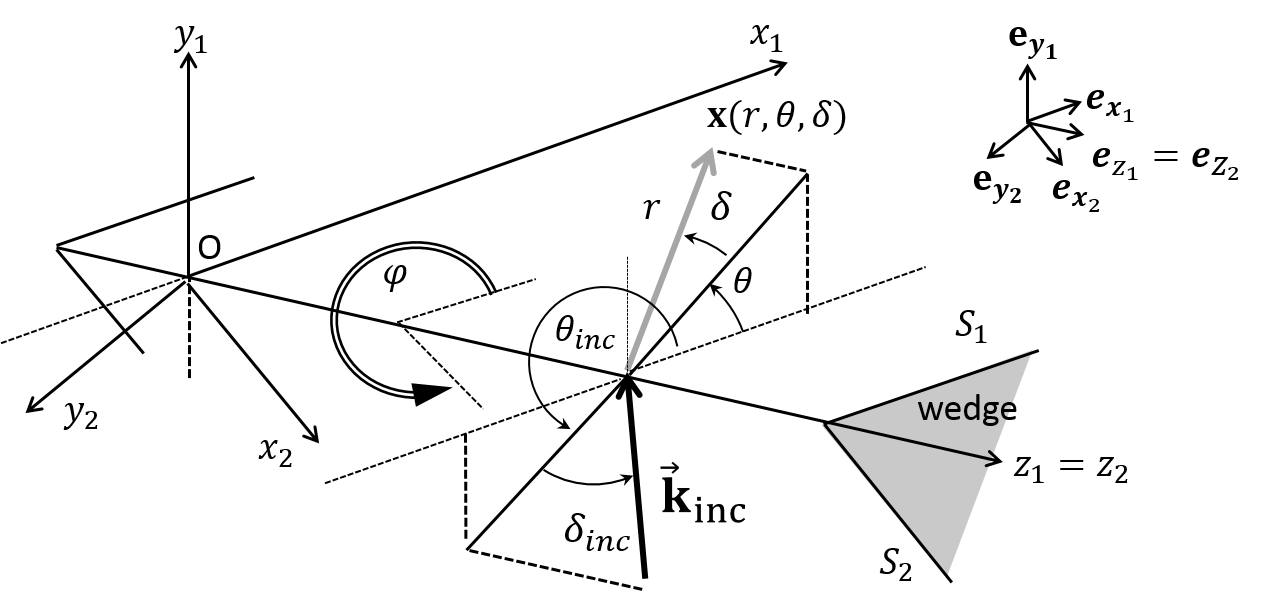
\includegraphics[width=\textwidth]{images/chapter4/wedge_3D.png}
\caption{Geometry of the problem}
\label{diedre_coords}
\end{figure}

Let us consider the problem of an elastic wave diffracted by a stress-free wedge delimited by faces $\mathcal{S}_1$ and $\mathcal{S}_2$. The geometry of the problem is shown on Fig.~\ref{diedre_coords}. The domain $\Omega$ is the inside of the wedge, defined by :
\begin{equation}
\Omega=\{ (r\cos \theta \cos \delta, r \sin \theta \cos \delta, r \sin \delta)\, \backslash \, \theta \in \rbrack 0, \varphi \lbrack, \, \delta \in \rbrack -\frac{\pi}{2}, \frac{\pi}{2} \lbrack \}
\end{equation}
%et sa surface
%$$ \mathcal{S}=\mathcal{S}_1 \cup \mathcal{S}_2 $$

The incident wave is a plane wave of the form
\begin{equation}
\mathbf{u}^{inc}(\mathbf{x},t)=\mathbf{A}_{\alpha}e^{i(\mathbf{k}_{\alpha}^{inc}\cdot \mathbf{x}-\omega t)}
\end{equation}
where $\mathbf{A}_{\alpha}$ is the amplitude vector of the incident wave and $\mathbf{k}_{\alpha}^{inc}$ is the incident wave vector. The type of the incident wave is denoted $\mathbf{k}_{\alpha}^{inc}$ (L for a longitudinal wave, TH for transverse horizontal and TV for transverse vertical). $(\mathbf{x}_1,\mathbf{y}_1, \mathbf{z}_1)$ is a Cartesian coordinate system associated to face $\mathcal{S}_1$. In this system, the incident wave vector is given by :
\begin{equation}
\mathbf{k}_{\alpha}^{inc}=\frac{\omega}{c_{\alpha}} \begin{pmatrix}
\cos\theta_{inc} \cos \delta_{inc} \\ \sin\theta_{inc} \cos \delta_{inc} \\
\sin \delta_{inc}
\end{pmatrix}
\end{equation}
As always, $c_L$ is the velocity of longitudinal waves and $c_T$ is the velocity of transverse waves.

The amplitude vector can be directed by three different and two-by-two orthogonal vectors, depending on the incident wave's polarization. These unit polarization vectors are noted $\hat{i}_*$, where $*=L, TH, TV$ and are given by Achenbach \cite{Achenbach} :
\begin{equation}
\hat{i}_L = \begin{pmatrix}
\cos\theta_{inc} \cos \delta_{inc} \\ \sin\theta_{inc} \cos \delta_{inc} \\
\pm \sin \delta_{inc}
\end{pmatrix}
\hfill
\hfill
\hat{i}_{TV} = \begin{pmatrix}
\mp\cos\theta_{inc} \sin \delta_{inc} \\ \mp\sin\theta_{inc} \sin \delta_{inc} \\
\cos \delta_{inc}
\end{pmatrix}
\hfill
\hfill
\hat{i}_{TH} = \begin{pmatrix}
-\sin\theta_{inc} \\ \cos\theta_{inc} \\
0
\end{pmatrix}
\label{ivec}
\end{equation}
where the top sign gives the polarization of an incident wave and the bottom sign gives the polarization of a diffracted wave.

In all the following, vectors are expressed in the coordinate system $(\mathbf{x}_1,\mathbf{y}_1, \mathbf{z}_1)$, except when explicitly mentioned otherwise. For a homogeneous, isotropic material, the linear elasticity equation solved by the displacement field $\mathbf{u}$ is 
\begin{equation}
\underline{\mu} \Delta \mathbf{u} + (\underline{\lambda}+\underline{\mu})\nabla \nabla \mathbf{u} = \rho \frac{\partial^2 \mathbf{u}}{\partial t^2}
\label{C4:Elasticitelin}
\end{equation}
On each of the wedge faces, the displacement field verifies the zero-stress boundary conditions, expressed as :
\begin{equation}
(\underline{\lambda} \nabla \mathbf{u} .\mathbf{\mathbb{I}_3}+2\underline{\mu} \mathbf{\varepsilon} (\mathbf{u})).\mathbf{n}=0
\label{C4:stressfree}
\end{equation}
where $\mathbf{\mathbb{I}_3}$ is the identity matrix of the third order, $n$ is the inward facing normal to the wedge face ($n=\mathbf{y}_1$ on $\mathcal{S}_1$  and $n=\mathbf{y}_2$ on $\mathcal{S}_2$) and $\underline{\lambda}, \underline{\mu}$ are the Lamé coefficients of the considered elastic medium. The expression of the deformations tensor is :
\begin{equation}
\mathbf{\varepsilon}(\mathbf{u})=\frac{1}{2} \begin{pmatrix}
2\dfrac{\partial u_1}{\partial x_1} & \dfrac{\partial u_1}{\partial y_1}+\dfrac{\partial u_2}{\partial x_1}&\dfrac{\partial u_1}{\partial z}+\dfrac{\partial u_3}{\partial x_1} \\
\dfrac{\partial u_1}{\partial y_1}+\dfrac{\partial u_2}{\partial x_1}&2\dfrac{\partial u_2}{\partial y_1}&\dfrac{\partial u_2}{\partial z}+\dfrac{\partial u_3}{\partial y_1} \\
\dfrac{\partial u_1}{\partial z}+\dfrac{\partial u_3}{\partial x_1} &\dfrac{\partial u_2}{\partial z}+\dfrac{\partial u_3}{\partial y_1} & 2\dfrac{\partial u_3}{\partial z}
\end{pmatrix}
\end{equation}
Kamotski and Lebeau \cite{KamotskiLebeau} have proven existence and uniqueness of the solution to this problem in the 2D the case. We will suppose that their demonstration is still valid in the 3D case.

From hereon after, bold characters will be reserved to matrices in order to simplify notations. The solutions being time harmonic, the factor $e^{-i\omega t}$ will be implied but omitted everywhere. Furthermore, since there is no obstacle to propagation in the $z$ direction, $e^{i\frac{\omega}{c_{\alpha}}\sin\delta_{inc}z}$ is also a common factor to all the terms which appear in the solution.

The total field is written as the sum of an incident field $u^{inc}$ and a scattered field $u_0$
\begin{equation}
u=u_0+u^{inc}
\label{C4:scat}
\end{equation}

The dimensionless problem is obtained by applying the following variable change :
\begin{equation}
u_0(x,y,z)=v\left( \frac{\omega}{c_L} x, \frac{\omega}{c_L} y \right)e^{i\nu_{\beta}\sin\delta_{\beta}z}
\label{C4:adiming}
\end{equation}
where $\delta_{\beta}$ is the angle of Snell's cone of diffraction, the dimensionless Lamé parameters $\lambda,\mu$ are given by \eqref{LameAdim} and parameters $\nu_L$ and $\nu_T$ are defined by \eqref{nuLnuT}. Since $e^{i\nu_{\alpha}\sin\delta_{inc}z}$ is a common factor to all the terms of the solution, we can deduce Snell's law of diffraction :
\begin{equation}
\nu_{\alpha}\sin\delta_{inc}=\nu_{\beta}\sin\delta_{\beta}
\label{C4:Snelldiff}
\end{equation}
To simplify notations, we define the following parameter $\tau$ is defined by :
\begin{equation}
\tau=\nu_{\alpha}\sin\delta_{\alpha}
\label{deftau}
\end{equation}
Note that we therefore always have $\tau \in \lbrack -\nu_{\alpha}, \nu_{\alpha} \rbrack$. $u_0$'s $z$-dependency is entirely contained in the factor $e^{i\tau z}$ which will be implied but omitted in all the following.

Substituting \eqref{C4:scat} and \eqref{C4:adiming} into \eqref{C4:Elasticitelin} and \eqref{C4:stressfree} yields the dimensionless problem
\begin{eqnarray}
(\mathcal{P}^*) \hspace{2em} \left\{
\begin{array}{lr}
(E+1)v=0 & (\Omega) \\
Bv=-Bv_{\alpha}^{inc} & (\mathcal{S})
\end{array}
\right.
\label{C4:Padim}
\end{eqnarray}
where $(v_1,v_2,v_3)$ are the components of vector $v$ :
\begin{equation}
Ev=\mu (\Delta v -\tau^2 v)+(\lambda+\mu)
\begin{pmatrix}
\frac{\partial^2 v_1}{\partial x^2}+\frac{\partial^2 v_2}{\partial x \partial y} + i\tau\frac{\partial v_3}{\partial x} \\
\frac{\partial^2 v_1}{\partial x \partial y}+\frac{\partial^2 v_2}{\partial y^2}+ i\tau\frac{\partial v_3}{\partial y}\\
i\tau\left( \frac{\partial v_1}{\partial x}+\frac{\partial v_2}{\partial y}\right)-\tau^2 v_3
\end{pmatrix}
\label{C4:Eadim}
\end{equation}
and
\begin{equation}
Bv=\begin{pmatrix}
\mu \left(\frac{\partial v_x}{\partial y}+\frac{\partial v_y}{\partial x}\right) \\
\frac{\partial v_y}{\partial y}+\lambda\left( \frac{\partial v_x}{\partial x}+i\tau v_z\right)\\
\mu \left(\frac{\partial v_z}{\partial y}+i\tau v_y\right)
\end{pmatrix}
\label{C4:Badim}
\end{equation}
where $E$ and $B$ are respectively the dimensionless linear elasticity operator and normal stress operator. The first equation of system \eqref{C4:Padim} is the dimensionless version of the linear elasticity equation and the second equation is the dimensionless version of the stress-free boundary conditions.

\section{Integral formulation of the solution}
As for the previous cases, the first step in solving problem $(\mathcal{P}^{\alpha})$ is to formulate the solution as an integral. 
\subsection{Limiting absorption principle}
The limiting absorption principle is applied to $(\mathcal{P}^{\alpha})$. This means that it is considered as a special case $(\varepsilon=0)$ of the problem
\begin{eqnarray}
(\mathcal{P}^*_{\epsilon}) \hspace{2em} \left\{
\begin{array}{lr}
(E+e^{-2i\epsilon})v^{\epsilon}=0 & (\Omega) \\
Bv^{\epsilon}=-Bv_*^{inc} & (\mathcal{S})
\end{array}
\right.
\label{C4:Pabs}
\end{eqnarray}
Following Kamotski and Lebeau \cite{KamotskiLebeau}, we will once again suppose that the solution can be expressed as the sum of two contributions, corresponding to each of the wedge faces :
\begin{equation}
v^{\epsilon}=v_1^{\epsilon}+v_2^{\epsilon}
\label{C4:v1+v2}
\end{equation}
where functions $v_j^{\epsilon}$ are now defined on all of  $\mathbb{R}^3$ by
\begin{equation}
v_j^{\epsilon}=-(E+e^{-2i\epsilon})^{-1} \begin{bmatrix}
\begin{pmatrix}
\alpha_j \\
\beta_j \\
\gamma_j
\end{pmatrix}
\otimes \delta_{\mathcal{S}_j}
\end{bmatrix}
\label{C4:vjdef}
\end{equation}
Distributions $\alpha_j,\beta_j, \gamma_j $ are unknown and are supposed to belong to the special call $\mathcal{A}$ defined in \ref{defClassA}. We can now define the outgoing solution of $(\mathcal{P}^{\alpha})$ analogously to the 2D case :
\begin{definition}
	 v is called an outgoing solution of equation \eqref{C4:Padim} if v is a solution of the form
	\begin{equation}
	\label{C4:decomposition}
	v=v_1|_{\Omega}+v_2|_{\Omega}
	\end{equation}
	where, for $j=1,2$ :
	\begin{equation}
	\label{C4:inv_potentiels}
	v_j=-\lim_{\epsilon \to 0} (E+e^{-2i\epsilon})^{-1} \begin{bmatrix}
\begin{pmatrix}
\alpha_j \\
\beta_j \\
\gamma_j
\end{pmatrix}
\otimes \delta_{\mathcal{S}_j}
\end{bmatrix}
	\end{equation}
	where $\alpha_j,\beta_j,\gamma_j \in \mathcal{A}$. %and where $\delta_{\mathcal{S}_1}$ and $\delta_{\mathcal{S}_2}$ sont les distributions de Dirac associés aux faces $\mathcal{S}_1$ et $\mathcal{S}_2$ du dièdre respectivement.
\end{definition}
The following theorem was proved by Kamotski and Lebeau \cite{KamotskiLebeau} in the 2D case. We will suppose that their proof can be adapted to the 3D case and that the theorem is still true.
\begin{theorem}
Equation \eqref{C4:Padim} admits a unique outgoing solution.
\end{theorem}
Nous that the outgoing solution has been defined, we will derive an integral formulation of this solution.

\subsection{Integral formulation}
The two-sided Fourier transform and its inverse transform are defined by \eqref{fullfourierdef}. The first step in determining an integral formulation of the solution is to apply the two-sided Fourier transform to \eqref{C4:vjdef}. This possible because all the distributions that appear in this equation are tempered distributions and they therefore admit a Fourier transform. We then have :
\begin{equation}
\hat{v}^{\epsilon}_j(\xi,\eta)=(\mathbf{M}-e^{-2i\epsilon}\mathbf{\mathbb{I}_3})^{-1}\Sigma_j(\xi)
\label{C4:matMvjeps}
\end{equation}
where $\Sigma_j, j=1,2$  are the unknown spectral functions, defined by :
\begin{equation}
\Sigma_j(\xi,)=\begin{pmatrix}
\hat{\alpha_j}(\xi)\\ \hat{\beta_j}(\xi) \\ \hat{\gamma_j}(\xi)
\end{pmatrix}
\end{equation}
and where \textbf{M} is the two-sided Fourier transform of operator $E$. Its expression is :
\begin{equation}
\mathbf{M}(\xi,\eta)=
\begin{pmatrix}
\xi^2+\mu(\eta^2+\tau^2) & (\lambda+\mu)\xi \eta & (\lambda+\mu)\xi\tau \\
 (\lambda+\mu)\xi \eta & \eta^2+\mu(\xi^2+\tau^2) & (\lambda+\mu)\eta\tau \\
(\lambda+\mu)\xi\tau & (\lambda+\mu)\eta\tau & \tau^2+\mu(\xi^2+\eta^2) 
\end{pmatrix}
\label{C4:matM}
\end{equation}
Substituting $\lambda$ by $1-2\mu$ and $\mu$ by $1/\nu_T^2$, \eqref{C4:matM} yields
\begin{multline}
(\mathbf{M}-e^{-2i\epsilon}\mathbb{I}_3)^{-1}=\\
\frac{\begin{pmatrix}
\xi^2+\nu_T^2(\eta^2+\tau^2-e^{-2i\epsilon}) & (1-\nu_T^2)\xi \eta & (1-\nu_T^2)\xi \tau \\
(1-\nu_T^2)\xi \eta & \eta^2+\nu_T^2(\xi^2+\tau^2-e^{-2i\epsilon}) & (1-\nu_T^2)\tau \eta \\
(1-\nu_T^2)\xi \tau & (1-\nu_T^2)\tau \eta & \tau^2+\nu_T^2(\eta^2+\xi^2-e^{-2i\epsilon})
\end{pmatrix}}{(\xi^2+\eta^2+\tau^2-e^{-2i\epsilon})(\xi^2+\eta^2+\tau^2-\nu_T^2e^{-2i\epsilon})} 
\end{multline}

Finally, the integral formulation of $v_j$ is obtained by inverting the two-sided Fourier transform applied in \eqref{C4:matMvjeps} :
\begin{equation}
v_j^{\epsilon}(x_j,y_j)=\frac{1}{4\pi^2}\int_{\mathbb{R}^2} e^{i x_j\xi}\left( \int_{-\infty}^{+\infty}e^{iy_j\eta} (\mathbf{M}-e^{-2i\epsilon}\mathbf{\mathbb{I}_3})^{-1} \,d\eta \right) \Sigma_j(\xi) \,d\xi
 \label{C4:invdouble}
\end{equation}

The poles of $(\mathbf{M}-e^{-2i\epsilon}\mathbf{\mathbb{I}_3})^{-1}$ are located in $\eta=\pm \zeta_*^{\epsilon}(\xi)$, where $*=L,T$ and
\begin{equation}
\zeta_*^{\epsilon}(\xi)=\sqrt{e^{-2i\epsilon}\nu^2_*-(\xi^2+\tau^2)}
\end{equation}
Let us define $\nuti_*, *=L,T$ by
\begin{equation}
\nuti_*^{\epsilon}=\sqrt{e^{-2i\epsilon}\nu_*^2-\tau^2}
\label{defnutieps}
\end{equation}
If the incident wave is longitudinal, then $\nuti \in \mathbb{R}$. However, if the incident wave is transverse, then two cases may occur :
\begin{itemize}
	\item if $|\sin\delta_{inc}| \leq \frac{\nu_L}{\nu_T}$, then $\nuti_L \in \mathbb{R}$
	\item if $|\sin\delta_{inc}| >\frac{\nu_L}{\nu_T}$, then $\nuti_L=i\eta_L \in i\mathbb{R}$ 
\end{itemize} 
In any case,
\begin{equation}
\zeta_*^{\epsilon}(\xi)=\sqrt{\tilde{\nu}_*^{\epsilon^2}-\xi^2}
\end{equation}
The chosen branch cut is the one for which the square root's imaginary part is positive. It is defined by
 \begin{eqnarray}
 \zeta_*(\xi)=
 \left\{
 \begin{array}{lr}
 i\sqrt{\xi^2-\tilde{\nu}_*^2}& \mbox{si } |\xi| \geq |\nuti_*| \\
 -\sqrt{\tilde{\nu}_*^2-\xi^2}& \mbox{si } |\xi| \leq |\nuti_*|
 \end{array}
 \right.
 \label{defzeta}
 \end{eqnarray}
%La racine carrée complexe étant définie au signe près, $\sqrt{z}$ peut prendre deux valeurs distinctes pour $z$ fixé. C'est ce qu'on appelle les branches de coupure de la fonction. Les points de branchement sont les valeurs pour lesquelles ces branches se croisent (ici il s'agit de $\xi=\pm \tilde{\nu}_*^{\epsilon}$). Afin de bien définir $\zeta_*^{\epsilon}(\xi)$, on choisit la branche dont la partie imaginaire est positive. 

The inner integral of \eqref{C4:invdouble} is computed using Cauchy's residue theorem :
\begin{equation}
v_j^{\epsilon}(x_j,y_j)=\frac{i}{4\pi}e^{2i\epsilon}\int_{\mathbb{R}} e^{ix_j\xi}\sum_{*=L,T}e^{i|y_j|\zeta_*^{\epsilon}(\xi)}\mathbf{M_*}(\xi,\mbox{sgn }y_j)\Sigma_j(\xi)\,d\xi
\label{C4:vjeps}
\end{equation}
where $\mathbf{M_*}(\xi,t),$ and $t=\mbox{sgn}( y_j)$ are defined by
\begin{subequations}
\begin{equation}
\mathbf{M_L}(\xi,t)=\begin{pmatrix}
\frac{\xi^2}{\zeta_L^{\epsilon}} &t\xi & \frac{\xi\tau}{\zeta_L^{\epsilon}} \\
t\xi & \zeta_L^{\epsilon} & t\tau \\
\frac{\xi\tau}{\zeta_L^{\epsilon}}& t\tau & \frac{\tau^2}{\zeta_L^{\epsilon}}
\end{pmatrix}
\label{C4:MLeps}
\end{equation}
\begin{equation}
\mathbf{M_T^{\epsilon}}(\xi,t)=\begin{pmatrix}
\zeta_T^{\epsilon} +\frac{\tau^2}{\zeta_T^{\epsilon}}& -t\xi &-\frac{\xi\tau}{\zeta_T^{\epsilon}}\\
-t\xi & \frac{\xi^2+\tau^2}{\zeta_T^{\epsilon}}&-t\tau \\
-\frac{\xi\tau}{\zeta_T^{\epsilon}}&-t\tau&\zeta_T^{\epsilon} +\frac{\xi^2}{\zeta_T^{\epsilon}}
\end{pmatrix}
\label{C4:MTeps}
\end{equation}
\label{C4:M*eps}
\end{subequations}

These matrices can be computed in two different manners, providing a way to test this result. the first way to compute these matrices is by direct computation of the residues of matrix $(\mathbf{M}-e^{-2i\epsilon}\mathbf{\mathbb{I}_3})^{-1}$. The second option for computing these matrices is by computing the eigen vectors and eigen values of $\mathbf{M}$. %On trouve bien les mêmes résultats avec les deux méthodes.

The three eigen vectors of $\mathbf{M}$ and the corresponding eigen values are :
\begin{subequations}
\begin{equation}
    \mathbf{M}\begin{pmatrix}
    \xi \\ \eta \\ \tau 
    \end{pmatrix}
    =(\xi^2+\eta^2+\tau^2)\begin{pmatrix}
    \xi \\ \eta \\ \tau 
    \end{pmatrix}
\end{equation}
\begin{equation}
   \mathbf{M}\begin{pmatrix}
    -\eta \\ \xi \\ 0
    \end{pmatrix}
    =\frac{\xi^2+\eta^2+\tau^2}{\nu_T^2}\begin{pmatrix}
    \xi \\ \eta \\ \tau 
    \end{pmatrix} 
\end{equation}
\begin{equation}
   \mathbf{M}\begin{pmatrix}
    -\xi\tau \\ \eta\tau \\ \xi^2+\eta^2
    \end{pmatrix}
    =\frac{\xi^2+\eta^2+\tau^2}{\nu_T^2}\begin{pmatrix}
    -\xi\tau \\ \eta\tau \\ \xi^2+\eta^2
    \end{pmatrix} 
\end{equation}
\end{subequations}
These three vectors are linearly independent and constitute a vector basis of $\mathbb{C}^3$. This means that any vector of $\mathbb{C}^3$ can be expressed as a linear combination of these three vectors. Notably :
\begin{equation}
    \begin{pmatrix}
    \hat{\alpha}_j\\ \hat{\beta}_j\\ \hat{\gamma}_j
    \end{pmatrix}
    = \frac{\xi\hat{\alpha}_j+\eta\hat{\beta}_j+\tau\hat{\gamma}_j}{\xi^2+\eta^2+\tau^2}\begin{pmatrix}
    \xi \\ \eta \\ \tau 
    \end{pmatrix} + \frac{\xi\hat{\beta}_j-\eta\hat{\alpha}_j}{\xi^2+\eta^2} \begin{pmatrix}
    -\eta \\ \xi \\ 0
    \end{pmatrix} + \frac{(\xi^2+\eta^2)\hat{\gamma}_j-\tau(\xi\hat{\alpha}_j+\eta\hat{\beta}_j)}{(\xi^2+\eta^2)(\xi^2+\eta^2+\tau^2)} \begin{pmatrix}
    -\xi\tau \\ \eta\tau \\ \xi^2+\eta^2
    \end{pmatrix}
\end{equation}
This second computation method thus yields
\begin{equation}
v_j^{\epsilon}(x_j,y_j)=\frac{i}{4\pi}e^{2i\epsilon}\int_{\mathbb{R}} e^{ix_j\xi}\sum_{*=L,TH,TV}e^{i|y_j|\zeta_*^{\epsilon}(\xi)}\mathbf{M_*}(\xi,\mbox{sgn }y_j)\Sigma_j(\xi)\,d\xi
\label{C4:vjeps2}
\end{equation}
where $\mathbf{M_L}(\xi,t),$ is given by \eqref{C4:MLeps} and
\begin{subequations}
\begin{equation}
\mathbf{M_{TV}}(\xi,t)=\begin{pmatrix}
\frac{\xi^2\tau^2}{\zeta_T(\xi^2+\zeta^2)}&\frac{t\xi\tau^2}{\xi^2+\zeta_T^2}&\frac{-\xi\tau}{\zeta_T}\\
\frac{t\xi\tau^2}{\xi^2+\zeta_T^2}&\frac{\zeta_T\tau^2}{\xi^2+\zeta_T^2}&-t\tau\\
\frac{-\xi\tau}{\zeta_T}&-t\tau&\frac{\xi^2+\zeta_T^2}{\zeta_T}
\end{pmatrix}
\label{C4:MTVeps}
\end{equation}
\begin{equation}
\mathbf{M_{TH}}(\xi,t)=\left(1+\frac{\tau^2}{\xi^2+\zeta_T^2}\right)\begin{pmatrix}
\zeta_T&-t\xi&0\\
-t\xi&\frac{\xi^2}{\zeta_T}&0\\
0&0&0
\end{pmatrix}
\label{C4:MTHeps}
\end{equation}
\label{C4:M*eps2}
\end{subequations}
Note that $ \mathbf{M_T}=\mathbf{M_{TH}}+\mathbf{M_{TV}}$. Expressions \eqref{C4:vjeps} and \eqref{C4:vjeps2} are equivalent.

Integral \eqref{C4:vjeps} is well defined for all values of $\epsilon \in \rbrack 0, \pi \lbrack $, since for these values of $\epsilon$, the integration contour never crosses the branch points of the integrand, which are located at $\xi=\pm \tilde{\nu}_*^{\epsilon}$, outside of the real axis.

According to Croisille et Lebeau \cite{CroisilleLebeau}, convergence in the 2D case is verified for $\epsilon \rightarrow 0$. We will suppose that this is still the case in 3D. The deformation contour $\mathbb{R}$ is deformed into contour $\Gamma_{0}$, visible on Fig.~\ref{C4:Gamma0_noncr} in the case where $\nuti_L\in\mathbb{R}$ and on Fig.~\ref{C4:Gamma0_cr} in the other case. This way the branch points of the integrand are avoided.

In all the following, superscript $\epsilon=0$ will be omitted in order to alleviate notations. Finally:
\begin{equation}
v_j(x_j,y_j)=\frac{i}{4\pi}\int_{\Gamma_0} e^{ix_j\xi}\sum_{*=L,T}e^{i|y_j|\zeta_*(\xi)}\mathbf{M_*}(\xi,\mbox{sgn }y_j)\Sigma_j(\xi)\,d\xi
\label{C4:vj0}
\end{equation}

\begin{figure}
\centering
\begin{subfigure}[b]{0.45\textwidth}
\begin{tikzpicture}
\node at (0,0) {$\times$};
\node at (0.35,0.35) {$0$};
\node at (2.25,0) {$\times$}; % Pole
\node at (1.5,0) {$\times$}; %pole
\node at (1.5,-0.45) {$\tilde{\nu}_L$};
\node at (2.25,-0.45) {$\tilde{\nu}_T$};
\node at (-1.5,0) {$\times$};
\node at (-2.25,0) {$\times$};
\node at (-1.5,0.45) {$-\tilde{\nu}_L$}; %pole
\node at (-2.25,0.45) {$-\tilde{\nu}_T$}; %pole
\node at (3.25,0.38) {$(\Gamma_0)$};
\node at (3.7,-0.38) {$\xi_1$};
\node at (0.38,2.25) {$\xi_2$};
%\draw[ thick, ->] (-2.5,-0.5) arc (180:235:1);
%\node at (-2.7,-0.9) {$F_1$};
%\draw[ thick, ->] (2.5,0.5) arc (0:45:1); %ici c'est les fleches 
%\node at (2.7,0.9) {$F_2$};
\draw[thick,black,yshift=0pt,decoration={markings,
mark=at position 1 with {\arrow{stealth}}},
postaction={decorate}](0,-2.5) -- (0,2.5);
\draw[thick,black,yshift=0pt,
decoration={ markings,  % This schema allows for fine-tuning the positions of arrows 
      mark=at position 0.1 with {\arrow{latex}},
      mark=at position 0.6 with {\arrow{latex}},
      mark=at position 0.9 with {\arrow{latex}},
      mark=at position 1 with {\arrow{stealth}}},
      postaction={decorate}]
      (-4,0) -- (-2.5,0)  arc (-180:0:0.25) -- (-1.75,0)  arc (-180:0:0.25)  -- (1.25,0)arc (180:0:0.25)  -- (2,0)arc (180:0:0.25) -- (3.75,0); % ca c'est l'axe
\end{tikzpicture}
\caption{Contour $\Gamma_0$ in the case where $\nuti_L \in \mathbb{R}$}
\label{C4:Gamma0_noncr}
\end{subfigure}
\hfill
\centering
\begin{subfigure}[b]{0.45\textwidth}
\begin{tikzpicture}
\node at (0,0) {$\times$};
\node at (0.35,0.35) {$0$};
\node at (2.25,0) {$\times$}; %pole
\node at (2.25,-0.45) {$\tilde{\nu}_T$};
\node at (-2.25,0) {$\times$};
\node at (-2.25,0.45) {$-\tilde{\nu}_T$}; %pole
\node at (3.5,0.38) {$(\Gamma_0)$};
\node at (0,1.5) {$\times$};
\node at (0.45, 1.5) {$\nuti_L$};
\node at (0,-1.5) {$\times$};
\node at (0.45,-1.5) {$-\nuti_L$};
\node at (3.9,-0.38) {$\xi_1$};
\node at (0.38,2.25) {$\xi_2$};
\draw[thick,black,yshift=0pt,decoration={markings,
mark=at position 0.99 with {\arrow{stealth}}},
postaction={decorate}](0,-2.5) -- (0,2.5);
\draw[thick,black,yshift=0pt,
decoration={ markings,  % This schema allows for fine-tuning the positions of arrows 
      mark=at position 0.1 with {\arrow{latex}},
      mark=at position 0.6 with {\arrow{latex}},
      mark=at position 0.9 with {\arrow{latex}},
      mark=at position 0.99 with {\arrow{stealth}}},
     postaction={decorate}]
      (-3.75,0) -- (-2.5,0)  arc (-180:0:0.25) -- (2,0)arc (180:0:0.25) -- (4,0); % ca c'est l'axe
\end{tikzpicture}
\caption{Contour $\Gamma_0$ in the case where $\nuti_L \in i\mathbb{R}$}
\label{C4:Gamma0_cr}
\end{subfigure}
\caption{Contour $\Gamma_0$ in the complex plane $\xi=\xi_1+i\xi_2$}
\label{C4:Gamma0}
\end{figure}


\subsection{Far field approximation}
$x=(x_1,y_1,z_1)=(r\cos\theta\cos\delta,r\sin\theta\cos\delta,r\sin\delta)$ is an observation point, indexed by its spherical coordinates, visible on Fig.~\ref{diedre_coords}. According to \eqref{C4:adiming},the scattered field at point $P$ is :
\begin{equation}
u_0(x_1,y_1,z)=v(\frac{\omega}{c_L}r\cos\theta\cos\delta,\frac{\omega}{c_L}r\sin\theta\cos\delta)e^{ik_{\beta}\sin\delta_{\beta}z}
\end{equation}
The far field parameter is $R=\frac{\omega r}{c_L}$. The aim is to determine the asymptotic behavior of $v(R\cos\theta\cos\delta,R\sin\theta\cos\delta)$ when $R\rightarrow +\infty$.The first step is to apply the change following of variables in integral $v_1$ :
\begin{equation}
\begin{split}
\xi&=\tilde{\nu}_*\cos\lambda \\
d\xi&=-\tilde{\nu}_*\sin\lambda\, d\lambda
\end{split}
\label{C4:changevar2}
\end{equation}
yielding
\begin{equation}
v_1(r,\theta,\delta)=\frac{i}{4\pi} \int_{C_0}\sum_{*=L,T}\tilde{\nu}_*^2 e^{i\tilde{\nu}_*R\cos\delta\cos(\lambda+\bar{\theta})}\mathbf{ P_*}(\lambda,t)\Sigma_1(\tilde{\nu}_*\cos\lambda) \, d \lambda
\label{C4:v1C0}
\end{equation}
where $\bar{\theta}$ has been defined by \eqref{obs} and
\begin{equation}
\mathbf{P_L}(\lambda,t)=
\begin{pmatrix}
\cos^2\lambda & -t\cos\lambda\sin\lambda &\frac{\tau}{\tilde{\nu}_L} \cos\lambda \\
-t\cos\lambda\sin\lambda & \sin^2\lambda&-t\frac{\tau}{\tilde{\nu}_L}\sin\lambda \\
\frac{\tau}{\tilde{\nu}_L} \cos\lambda&-t\frac{\tau}{\tilde{\nu}_L}\sin\lambda&\frac{\tau^2}{\tilde{\nu}_L^2}
\end{pmatrix}
\end{equation}
and
\begin{equation}
\mathbf{P_T}(\lambda,t)=
\begin{pmatrix}
\sin^2\lambda+\frac{\tau^2}{\tilde{\nu}_T^2} & t\cos\lambda\sin\lambda &-\frac{\tau}{\tilde{\nu}_T}\cos\lambda \\
t\cos\lambda\sin\lambda & \cos^2\lambda+\frac{\tau^2}{\tilde{\nu}_T^2}&t\frac{\tau}{\tilde{\nu}_T}\sin\lambda \\
-\frac{\tau}{\tilde{\nu}_T}\cos\lambda&t\frac{\tau}{\tilde{\nu}_T}\sin\lambda&1
\end{pmatrix}
\end{equation}
$t=\mbox{sgn} \sin\theta$ and contour $C_0$ is visible on Fig.~\ref{C4:steepestcontour}.

Note that in the case $\nuti_L =i\eta_L \in i\mathbb{R}$, variable change \eqref{C4:changevar2} produces an evanescent term :
\begin{equation}
\begin{split}
v_1(r,\theta,\delta)&=-\frac{i}{4\pi} \int_{C_0^L}\eta_L^2 e^{-\eta_L R\cos\delta\cos(\lambda+\bar{\theta})}\mathbf{ P_L}(\lambda,t)\Sigma_1(i\eta_L\cos\lambda) \, d\lambda\\
&+\frac{i}{4\pi} \int_{C_0}\tilde{\nu}_T^2 e^{i\nuti_T R\cos\delta\cos(\lambda+\bar{\theta)})}\mathbf{ P_T}(\lambda,t)\Sigma_1(\tilde{\nu}_T\cos\lambda) \, d\lambda
\end{split}
\label{C4:v1C0evan}
\end{equation}
where contour $C_0^L$ is visible on Fig.~\ref{C4:steepestcontour}. The exponential term in the first integral of \eqref{C4:v1C0evan} is $e^{-\eta_L R\cos\delta\cos(\lambda+\bar{\theta})}$, where $\eta_L>0$, $R>0$ and $\cos\delta>0$. Furthermore, for $\lambda :\in C_0^L$, we have :
\begin{equation}
\lambda=-\left(\dfrac{\pi}{2}^+\right)+i\lambda_2
\end{equation}
where the notation $\dfrac{\pi}{2}^+$ refers to a real number which tends to $\frac{\pi}{2}$ with superior values and $\lambda_2=\rm Im(\lambda)$. This yields
\begin{equation}
\cos(\lambda+\bar{\theta})=\cos(\bar{\theta}-\dfrac{\pi}{2})\cosh\lambda_2-i\sin(\bar{\theta}-\dfrac{\pi}{2})\sinh\lambda_2
\end{equation}
Having $\bar{\theta} \in \lbrack 0,\pi \rbrack$, we have $\cos(\bar{\theta}-\dfrac{\pi}{2})=\sin\bar{\theta}\leq 0$ and 
\begin{equation}
|e^{-\eta_L R\cos\delta\cos(\lambda+\bar{\theta})}|=e^{-\eta_L R\cos\delta\sin\bar{\theta}\cosh\lambda_2}
\end{equation}
The amplitude of the integrand in the first integral of \eqref{C4:v1C0evan} decreases exponentially as the distance from the edge grows. %This means that it is an evanescent term.

\begin{figure}
\centering
\begin{tikzpicture}
	\draw[step=1.5cm,gray,very thin,dashed](-2.5,-2.7)grid(3.7,3.7);
	\draw[thin, decoration={ markings,  
		mark=at position 1 with {\arrow{stealth}}},
	postaction={decorate}] (-2.5,0)  -- (3.7,0) node[above]{$\lambda_1$};
	\draw[thin, decoration={ markings,  
		mark=at position 1 with {\arrow{stealth}}},
	postaction={decorate}](0,-2.5)--(0,3.5) node[left]{$\lambda_2$};

	\node at (2.8,-0.2) {$\pi$};
	\node at (-0.2,0.2) {$0$};
	\node at (0.92,0.5) {$\lambda_s$};
	\node at (3,3.1) {$C_0$};
	\node at (1.9,3.1) {$\gamma_{\theta}$};
	\node at (-2.0,3.3) {$C_0^L$};
	
	\draw[black,very thick, decoration={ markings,  
		mark=at position 0.2 with {\arrow{latex}},
		mark=at position 0.8 with {\arrow{latex}}},
	postaction={decorate}] (-1.7,3.5)--(-1.7,-2.5);
	
	\draw[black,very thick][domain=0:3.5] plot({2*pi/7 + acos(1/cosh(\x))*pi/180},\x);
	\draw[black,very thick, decoration={ markings,  
		mark=at position 0.2 with {\arrow{latex}}},
	postaction={decorate}][domain=0:-2.8] plot({2*pi/7 - acos(1/cosh(\x))*pi/180},\x);
	
	\draw[very thick,black,%xshift=0pt,
	decoration={ markings,  
		mark=at position 0.8 with {\arrow{latex}}},
	postaction={decorate}]
	(0.2,0.2) arc (0:-90:0.4) -- (-0.2,-3); 
	
	\draw[very thick,black,%yshift=0pt,
	decoration={ markings, mark=at position 0.5 with {\arrow{latex}}}, postaction={decorate}]
	(pi-0.57,0.2) -- (0.2,0.2);

	\draw[very thick,black,%xshift=0pt,
	decoration={ markings,  
		mark=at position 0.5 with {\arrow{latex}}},
	postaction={decorate}]
	(pi-0.4,3.2) -- (pi-0.4,0.4) arc (0:-90:0.2) ;

	\end{tikzpicture}
	\caption{Contours $C_0$ and $\gamma_{\theta}$ in the complex plane $\lambda=\lambda_1+i\lambda_2$. The stationary phase points are noted $\lambda_s$.}
	\label{C4:steepestcontour}
\end{figure}

The far-field evaluation of the integral is obtained by applying the steepest descent method, presented in appendix \ref{PhaseStationnaire}, to \eqref{C4:v1C0}. To do so, contour $C_0$ is deformed into contour $\gamma_{\theta}$, also visible in Fig.~\ref{C4:steepestcontour}. In the case $\nuti_L \in \mathbb{R}$, this leads to
\begin{equation}
v_1=v_1^{sing}+v_1^{diff}
\end{equation}
where $v_1^{sing}$ is the contribution of all the singularities of the spectral functions crossed during the deformation from $C_0$ to $\gamma_{\theta}$, corresponding to the reflected and head waves, and $v_1^{diff}$ is the contribution of the stationary phase point, corresponding to the diffracted wave and computed using \eqref{steepformula}. Only the contribution of the diffracted waves will be computed here. In order to simplify notations, we will note $\mathbf{P}_*(\lambda,1)=\mathbf{P}_*(\lambda)$ and $\mathbf{P}_*(\lambda,-1)=\mathbf{P}_*(-\lambda)$). The contribution of diffracted waves is 
\begin{equation}
v_1^{diff}(R\cos\theta,R\sin\theta)=\frac{e^{-i\pi/4}}{2\sqrt{2\pi}}\sum_{*=L,T}\tilde{\nu}_*^2\frac{e^{-i\tilde{\nu}_*R\cos\delta}}{\sqrt{\nuti_*R\cos\delta}}\mathbf{P_*}(\pi-\theta)\Sigma_1(-\tilde{\nu}_*\cos\theta)
\end{equation}
Analogously,
\begin{equation}
v_2^{diff}(R\cos(\varphi-\theta),R\sin(\varphi-\theta))=\frac{e^{-i\pi/4}}{2\sqrt{2\pi}}\sum_{*=L,T}\tilde{\nu}_*^2\frac{e^{-i\tilde{\nu}_*R\cos\delta}}{\sqrt{\nuti_*R\cos\delta}}\mathbf{P_*}(\pi-(\varphi-\theta))\Sigma_1(-\tilde{\nu}_*\cos(\varphi-\theta))
\end{equation}

In the case where $\nuti_L=i\eta_L \in i\mathbb{R}$, the far-field evaluation is obtained by applying the steepest descent method, presented in appendix \ref{PhaseStationnaire}, to \eqref{C4:v1C0evan}. Contour $C_0$ is deformed into contour $\gamma_{\theta}$ and contour $C_0^L$ is deformed into contour $\gamma_{\theta}^L$. This leads to
\begin{equation}
v_1=v_1^{sing}+v_1^{diff}+v_1^{evan}
\end{equation}
where $v_1^{sing}$ is the contribution of all the singularities of the spectral functions crossed during the deformation from $C_0$ to $\gamma_{\theta}$, $v_1^{diff}$ is the contribution of the stationary phase point to the integral on $C_0$, corresponding to the diffracted wave, and $v_1^{evan}$ is the contribution of the integral on $C_0^L$, which decays exponentially as the far-field parameter $R$ grows, making it an evanescent wave. Once again, only the contribution of the diffracted waves will be computed here. Contribution $v_1^{diff}$ is computed using \eqref{steepformula} :
%. The contribution of evanescent waves is 
%\begin{equation}
%v^{evan}_1(R\cos\theta,R\sin\theta)= \sqrt{\frac{2\pi}{R\eta_L\cos\delta_{\beta}}} e^{-R\eta_L\cos\delta}\mathbf{P_L}(-\theta)\Sigma_1(i\eta_L\cos\theta)
%\end{equation}
%and the contribution of diffracted waves is :
\begin{equation}
v_1^{diff}(R\cos\theta,R\sin\theta)=\frac{e^{-i\pi/4}}{2\sqrt{2\pi}}\tilde{\nu}_T^2\frac{e^{-i\tilde{\nu}_TR\cos\delta}}{\sqrt{\nuti_TR\cos\delta}}\mathbf{P_T}(\pi-\theta)\Sigma_1(-\tilde{\nu}_T\cos\theta)
\end{equation}
Analogously,
%\begin{equation}
%v^{evan}_2(R\cos\theta,R\sin\theta)= \sqrt{\frac{2\pi}{R\eta_L\cos\delta_{\beta}}} e^{-R\eta_L\cos\delta}\mathbf{P_L}(-(\varphi-\theta))\Sigma_1(i\eta_L\cos(\varphi-\theta))
%\end{equation}
%and
\begin{equation}
v_2^{diff}(R\cos\theta,R\sin\theta)=\frac{e^{-i\pi/4}}{2\sqrt{2\pi}}\tilde{\nu}_T^2\frac{e^{-i\tilde{\nu}_TR\cos\delta}}{\sqrt{\nuti_TR\cos\delta}}\mathbf{P_T}(\pi-(\varphi-\theta))\Sigma_2(-\tilde{\nu}_T\cos(\varphi-\theta))
\end{equation}

In both cases, the diffraction coefficient is defined by
\begin{equation}
v_{\beta}^{diff}(R\cos\theta,R\sin\theta)=D_{\beta}^{\alpha}(\theta,\delta)\frac{e^{-i\nuti_{\beta}R\cos\delta_{\beta}}}{\sqrt{\nuti_{\beta}R\cos\delta_{\beta}}} v^{inc}(R\cos\theta,R\sin\theta) \hat{i}_{\beta}
\label{C4:coeffdiff}
\end{equation}
The total diffracted field is
\begin{equation}
v^{diff}=v_1^{diff}+v_2^{diff}
\end{equation}

Let us now isolate L, TH and TV diffracted waves in order to compute the corresponding diffraction coefficients. Using the expressions of the unit vectors given by \eqref{ivec}, the $\beta$ diffracted wave is given by $v^{diff}\cdot \hat{i}_{\beta}$. This yields :
\begin{equation}
D_{\beta}^{\alpha}(\theta,\delta)=\frac{e^{-i\pi/4}}{2\sqrt{2\pi}}\sum_{j=1,2}\nuti_{\beta}^2 \,{}^t \Sigma_j(-\nuti_{\beta}\cos\theta_j)\cdot\left(\mathbf{P}_{\beta}(\pi-\theta_j).\hat{i}_{\beta}\right)
\label{C4:Dbeta}
\end{equation}
where $\theta_1=\theta$ and $\theta_2=\varphi-\theta$.

In order to determine the field diffracted by a wedge illuminated by an incident plane wave, it is sufficient to compute the diffraction coefficient. This coefficient has been expressed in terms of two unknown functions called the spectral functions. The semi-analytical computation of these functions is presented in the following section

\section{Semi-analytical evaluation of the spectral functions}
The first step in computing the spectral functions is to determine a system of functional equations of which they are a solution. We will then show that these functions can be decomposed into two parts : a singular function, computed analytically, and a regular function, approached numerically.
\subsection{Functional equations}
In the previous section, the diffracted wave has been expressed in terms of two unknown functions called the spectral functions. In this subsection, a system of functional equations satisfied by these functions is determined. 

The first step in determining a system of functional equations verified by the spectral functions, is to substitute decomposition \eqref{C4:v1+v2} into the boundary conditions :
\begin{equation}
\left\{
\begin{matrix}
B \big( v_1(x_1,0)+v_2(x_2 \cos \varphi, x_2 \sin \varphi) \big) = -B \rm v_{\alpha}^{inc}|_{\mathcal{S}_1} \\
B \big( v_2(x_2,0)+v_1(x_1 \cos \varphi, x_1 \sin \varphi) \big) = -B \rm v_{\alpha}^{inc}|_{\mathcal{S}_2}
\end{matrix}
\right.
\label{C4:Bivi}
\end{equation}
Let us note $(v_j^1,v_j^2,v_j^3)$ the coordinates of $v_j$ in the Cartesian coordinate system $(x_j,y_j,z_j)$, where $(x_1,y_1,z_1)$ is the coordinate system associated with face $\mathcal{S}_1$ and $(x_2,y_2,z_2)$ is the coordinate system associated with face $\mathcal{S}_2$. These two coordinate systems are linked by (for $j=1,2$):
\begin{equation}
    \left\{
    \begin{matrix}
    x_j=\cos\varphi .x_{3-j}+\sin\varphi. y_{3-j}\\
    y_j=\sin\varphi .x_{3-j}-\cos\varphi .y_{3-j}\\
    z_j=z_{3-j}
    \end{matrix}
    \right.
    \label{C4:changerep}
\end{equation}
Applying \eqref{C4:changerep} to each line of \eqref{C4:Bivi} yields: 
\begin{equation}
\left\{
\begin{matrix}
B_1(v_1)+B_2(v_2)=-Bv_{\alpha}^{inc}|_{\mathcal{S}_1} \\
B_1(v_2)+B_2(v_1)=-Bv_{\alpha}^{inc}|_{\mathcal{S}_2}
\end{matrix}
\right.
\label{C4:b1v1+b2v2}
\end{equation}
where
\begin{equation}
B_1(v)=
\begin{pmatrix}
\mu \left( \frac{\partial v_1}{\partial y_1}+\frac{\partial v_2}{\partial x_1} \right) \\
\frac{\partial v_2}{\partial y_1}+\lambda \left( \frac{\partial v_1}{\partial x_1}+i\tau v_3 \right)\\
\mu \left( \frac{\partial v_2}{\partial z_1}+ \frac{\partial v_3}{\partial y_1}\right)
\end{pmatrix}
\label{C4:B1v1expl}
\end{equation}
and
\begin{equation}
B_2(v)=
\begin{pmatrix}
\mu \sin(2\varphi)\left( \frac{\partial v_1}{\partial x_2}-\frac{\partial v_2}{\partial y_2}\right)-\mu \cos(2\varphi)  \left( \frac{\partial v_1}{\partial y_2}+\frac{\partial v_2}{\partial x_2} \right)\\
(\lambda+2\mu \sin^2\varphi) \frac{\partial v_1}{\partial x_2}+(\lambda+2\mu \cos^2 \varphi)\frac{\partial v_2}{\partial y_2}-\mu \sin(2\varphi)  \left( \frac{\partial v_1}{\partial y_2}+\frac{\partial v_2}{\partial x_2} \right)+\lambda \frac{\partial v_3}{\partial z_2} \\
\mu\sin\varphi\left(\frac{\partial v_3}{\partial x_2}+\frac{\partial v_1}{\partial z_2} \right)-\mu\cos\varphi\left( \frac{\partial v_2}{\partial z_2} +\frac{\partial v_3}{\partial y_2} \right)
\end{pmatrix}
\label{C4:B2v2expl}
\end{equation}
Operator $B_1$ is obtained by projecting $B(v_1)$ onto $\mathcal{S}_1$. This is immediate because $v_1$ is defined on $\mathcal{S}_1$ and its components $(v_1^1,v_1^2,v_1^3)$ are expressed in the associated Cartesian coordinate system $(x_1,y_1,z_1)$. Operator $B_2$ is obtained by projecting $B(v_2)$ onto $\mathcal{S}_1$. This is done by projecting its components $(v_2^1,v_2^2,v_2^3)$ onto $\mathcal{S}_1$ and by expressing $(x_1,y_1,z_1)$ as functions of $(x_2,y_2,z_2)$, as $v_2$ is only defined on $\mathcal{S}_2$. This is done using \eqref{C4:changerep}. The second equation of system \eqref{C4:b1v1+b2v2} is obtained analogously to the first (operators are projected onto $\mathcal{S}_2$ instead of $\mathcal{S}_1$).

The functional equations system solved by the spectral functions is obtained by substituting the integral formulation \eqref{C4:vj0} of $v_1$ and $v_2$ into \eqref{C4:b1v1+b2v2}, evaluating the first equation at $x_1\geq 0, y_1=0$ and the second at $x_2\geq 0, y_2=0$ and applying the Fourier transform to the result. This yields :
\begin{equation}
\begin{split}
\int_0^{+\infty} e^{-ix\xi}B_1(v_1)(x)\,dx&=\frac{1}{2}\textbf{DM}(\Sigma_1)(\xi) \\
&=\frac{1}{2} \int_{\Gamma_0}\textbf{DM}(\xi,\zeta)\Sigma_1(\zeta)\,d\zeta
\end{split}
\label{C4:B1DM}
\end{equation}
where
\begin{equation}
\begin{split}
\textbf{DM}(\xi,\zeta)&=\frac{1}{2i\pi} \frac{1}{\xi-\zeta} \textbf{dm}(\zeta) \\
&=\frac{1}{2i\pi} \frac{1}{\xi-\zeta} \begin{pmatrix}
-1 & \frac{\zeta}{\zeta_T}(1-2\mu Q(\zeta)) & 0\\
-\frac{\zeta}{\zeta_L}(1-2\mu Q(\zeta))  & -1&-\frac{\tau}{\zeta_L}(1-2\mu Q(\zeta)) \\
0&\frac{\tau}{\zeta_T}(1-2\mu Q(\zeta)) &-1
\end{pmatrix}
 \end{split}
\label{C4:defDM}
\end{equation}
and
\begin{equation}
Q(\zeta) =\zeta_L\zeta_T+\zeta^2+\tau^2
\end{equation}
Evaluating $B_2(v_2)$ at $x_1\geq 0, y_1=0$ means is equivalent to evaluating $B_2(v_2)$ at $x_2=x\cos\varphi, y_2=x\sin\varphi, x\geq 0$. The Fourier transform of the second term is therefore
\begin{equation}
\begin{split}
\int_0^{+\infty} e^{-ix\xi}B_2(v_2)(x)\,dx&=\frac{1}{2}\textbf{TM}(\Sigma_2)(\xi) \\
&=\frac{1}{2} \int_{\Gamma_0}\textbf{TM}(\xi,\zeta)\Sigma_2(\zeta)\,d\zeta
\end{split}
\label{C4:B2TM}
\end{equation}
where
\begin{equation}
\textbf{TM}(\xi,\zeta)=\frac{1}{2i\pi}\sum_{*=L,TH,TV}D_*(\xi,\zeta)\textbf{tm}_*(\zeta,\mbox{sgn } \sin \varphi),
\label{C4:defTM}
\end{equation}
$t=$sgn sin $\varphi$,
\begin{equation}
D_*(\xi,\zeta)=\frac{1}{\xi-(\zeta \cos \varphi + \zeta_*(\zeta) |\sin \varphi|)},
\end{equation}
and the following matrices of rank 1 are defined :
\begin{equation}
\left\{
\begin{matrix}
\textbf{tm}_L(\zeta)=\left[ \frac{\zeta}{\zeta_L} f_L\,; \, tf_L\,;  \, \frac{\tau}{\zeta_L}f_L
\right] \\
f_L = \begin{pmatrix}
\mu \lbrack \cos(2\varphi)(2t\zeta\zeta_L)-\sin(2\varphi)(\zeta^2-\zeta_L^2) \rbrack\\
-\lambda+2\mu \lbrack \sin(2\varphi)(t\zeta\zeta_L)-\zeta^2\sin^2\varphi-\zeta^2_L\cos^2\varphi\rbrack\\
-2\mu\tau\lbrack \zeta\sin\varphi -t\zeta_L\cos\varphi\rbrack
\end{pmatrix}
\end{matrix}
\right. ,
\label{C4:tmL}
\end{equation}
\begin{equation}
\left\{
\begin{matrix}
\textbf{tm}_{TH}(\zeta)=\lbrack -tf_{TH}\,;\, \frac{\zeta}{\zeta_T}f_{TH}\,;\, 0 \rbrack\\
f_{TH}=\mu\left(1+\frac{\tau^2}{\zeta^2+\zeta_T^2}\right) \begin{pmatrix}
\sin(2\varphi)(2t\zeta\zeta_T)+\cos(2\varphi)(\zeta^2-\zeta_T^2)\\
\sin(2\varphi)(\zeta^2-\zeta_T^2)-\cos(2\varphi)(2t\zeta\zeta_T)\\
\tau\lbrack t\zeta_T\sin\varphi+\zeta\cos\varphi\rbrack 
\end{pmatrix}
\end{matrix}
\right.
\label{C4:tmTH}
\end{equation}
and
\begin{equation}
\left\{
\begin{matrix}
\textbf{tm}_{TV}(\zeta)=\lbrack \frac{\zeta\tau}{\zeta_T(\zeta^2+\zeta_T^2)}f_{TV}\,;\, \frac{t\tau}{\zeta^2+\zeta_T^2}f_{TV}\,;\, -\frac{1}{\zeta_T}f_{TV} \rbrack\\
f_{TV}=\mu\begin{pmatrix}
\tau\cos(2\varphi)(2t\zeta\zeta_T)-\tau\sin(2\varphi)(\zeta^2-\zeta_T^2)\\
2\tau\lbrack \sin(2\varphi)(t\zeta\zeta_T)-\zeta^2\sin^2\varphi-\zeta_T^2\cos^2\varphi\rbrack\\
\left(\tau^2-\zeta^2+\zeta_T^2\right)\lbrack t\zeta_T\cos\varphi-\zeta\sin\varphi \rbrack
\end{pmatrix}
\end{matrix}
\right.
\label{C4:tmTV}
\end{equation}
In the following, let us note for simplification:
\begin{equation}
\mathbf{tm}_T=\mathbf{tm}_{TH}+\mathbf{tm}_{TV}
\end{equation}

It has been checked that setting $\tau=0$ in the explicit expressions of $\mathbf{DM}$ and $\mathbf{TM}$ operators leads to the same expressions as those found in the previous chapter, concerning the 2D case.

Finally, the Fourier transform of the boundary conditions on the wedge faces its obtained by summing \eqref{C4:B1DM} and \eqref{C4:B2TM}. The right-hand side of the system is obtained by taking the Fourier transform of $-Bv_{\alpha}^{inc}|_{\mathcal{S}_j}, \; j=1,2$. The final system of functional equations solved by the spectral functions is 
\begin{equation}
\left\{
\begin{matrix}
\textbf{DM}(\Sigma_1)+\textbf{TM}(\Sigma_2)=\dfrac{W_1^{\alpha}}{\xi-\nu_{\alpha} \cos \theta_{inc}\cos\delta_{inc}} 
\\
\textbf{TM}(\Sigma_1)+\textbf{DM}(\Sigma_2)=\dfrac{W_2^{\alpha}}{\xi-\nu_{\alpha}\cos(\varphi-\theta_{inc})\cos\delta_{inc}}
\end{matrix}
\right.
\label{C4:equationsintegrales}
\end{equation}
where
\begin{eqnarray}
\begin{array}{lr}
W_1^L=-2\begin{pmatrix}
\mu\cos^2\delta_{inc}\sin(2\theta_{inc}) \\
1-2\mu(\cos^2\theta_{inc}\cos^2\delta_{inc}+\sin^2\delta_{inc})\\
\mu\sin(2\delta_{inc})\sin(\theta_{inc})
\end{pmatrix}\\
~\\
 W_2^L=-2\begin{pmatrix}
\mu\cos^2\delta_{inc}\sin(2\varphi-2\theta_{inc}) \\
1-2\mu(\cos^2(\varphi-\theta_{inc})\cos^2\delta_{inc}+\sin^2\delta_{inc})\\
\mu\sin(2\delta_{inc})\sin(\varphi-\theta_{inc})
\end{pmatrix}\\ 
~\\
W_1^{TV}=2\nu_T\mu\begin{pmatrix}
\frac{1}{2}\sin(2\theta_{inc})\sin(2\delta_{inc})
\\
\sin(2\delta_{inc})\sin^2\theta_{inc}\\
-\sin\theta_{inc}\cos(2\delta_{inc})
\end{pmatrix}~
W_2^{TV}=2\nu_T\mu\begin{pmatrix}
\frac{1}{2}\sin(2\varphi-2\theta_{inc})\sin(2\delta_{inc})
\\
\sin(2\delta_{inc})\sin^2(\varphi-\theta_{inc})\\
-\sin(\varphi-\theta_{inc})\cos(2\delta_{inc})
\end{pmatrix} \\
~
\\
W_1^{TH}=-2 \nu_T\mu \begin{pmatrix}
\cos\delta_{inc}\cos(2\theta_{inc})
\\
\sin(2\theta_{inc})\cos\delta_{inc}\\
\cos\theta_{inc}\sin\delta_{inc}
\end{pmatrix}
~
W_2^{TH}=2 \nu_T\mu \begin{pmatrix}
\cos\delta_{inc}\cos(2\varphi-2\theta_{inc})\\
\sin(2\varphi-2\theta_{inc})\cos\delta_{inc}\\
\cos(\varphi-\theta_{inc})\sin\delta_{inc}
\end{pmatrix}
\end{array}
\label{C4:Wj}
\end{eqnarray}

Thanks to these functional equations, the spectral functions can be decomposed into two parts : a singular function and a regular function. The evaluation of each of these parts is described in the following.

\subsection{Singular part}
\label{C4:singpart}
The first step in evaluating the spectral functions is to determine their poles and corresponding residues. As in the previous chapters, this is done using to a recursive procedure, in which the following translation appears (for $*=L,T$) :
\begin{equation}
\begin{split}
T_*(\xi)&=\xi \cos \varphi+\zeta_*(\xi)\sin \phiti \\
&=\tilde{\nu}_*\cos(\theta+\tilde{\varphi})
\end{split}
\end{equation}
where $\phiti$ is defined in \eqref{phitilde}. This translation operator is defined on subspace $\Omega_*^+$, represented on Fig.~\ref{C4:domega0} :
\begin{equation}
\xi \in \Omega_*^+= \{ \xi=\tilde{\nu}_* \cos \theta, \; 0 \leq \mbox{Re} \theta < \pi-\tilde{\varphi} \}
\label{C4:defOmega0}
\end{equation}
In order to determine the action of operator $\mathbf{DM}$ on a simple pole, contour $\Gamma_0$ in \eqref{C4:B1DM} is deformed into contour $\Gamma_1$, visible in Fig.~\ref{C4:gamma1noncr} for the case $\nuti_L \in \mathbb{R}$ and in Fig.~\ref{C4:gamma1cr} for the case $\nuti_L \in i\mathbb{R}$. In both cases, Cauchy's residue theorem is applied, yielding for $V \in \mathbb{C}^3$, Im$z\geq 0, \, z \notin \{\pm\tilde{\nu}_L,\pm\tilde{\nu}_T \}$, Im$\xi <0 $ with $z\in \mathbb{C} \backslash  \rbrack - \infty, -\nuti_L \rbrack$ if $\noncr$ and $ z\in \mathbb{C} \backslash ( \, \rbrack - \infty, -\nuti_T \rbrack \cup \lbrack \nuti_L,+i\infty \lbrack \,)$ if $\crit$ :
\begin{equation}
\int_{\Gamma_0} \textbf{DM}(\xi,\zeta).\frac{V}{\zeta-z}\,d\zeta = \frac{\textbf{dm}(z).V}{\xi-z}+D_p(z,\xi),
\label{C4:GaussDM}
\end{equation}
where
\begin{equation}
D_p(z,\xi)= \int_{\Gamma_1} \frac{\textbf{DM}(\xi,\zeta)}{\zeta-z}\,d\zeta
\label{C4:defDp}
\end{equation}

\begin{figure}
\centering
\begin{tikzpicture}
\node at (0,0) {$\times$};
\node at (0,0.35) {$0$};
\node at (2,0) {$\times$}; % Pole
\node at (4,0) {$\times$}; %pole
\node at (2,-0.36) {$\tilde{\nu}_L$};
\node at (4,-0.36) {$\tilde{\nu}_T$};

\node at (-2,0) {$\times$};
\node at (-4,0) {$\times$};
\node at (-2,0.36) {$-\tilde{\nu}_L$}; %pole
\node at (-4,0.36) {$-\tilde{\nu}_T$}; %pole
\node at (-3,-0.6) {$\Gamma_1$};

\draw[dashed, decoration={markings,
 mark=at position 1.0 with {\arrow{latex}}},
      postaction={decorate}] (-1.5,0) -- (6,0);
      
\draw[ thick, ->] (3.0,0.3) arc (0:45:1); %ici c'est les fleches 
  

\draw[thick, black, yshift=0pt,
decoration={ markings,  % This schema allows for fine-tuning the positions of arrows 
      mark=at position 0.1 with {\arrow{latex}},
      mark=at position 0.9 with {\arrow{latex}}},
      postaction={decorate}]
      (-6,0) -- (-4.25,0)  arc (-180:0:0.25) -- (-2.25,0)  arc (-180:0:0.25) -- (-1.75,0) arc(-90:90:0.5)  -- (-6,1);
\end{tikzpicture}
\caption{Contour $\Gamma_1$ in the case $\noncr$. The arrow shows the deformation of contour $\Gamma_0$ into $\Gamma_1$.}
\label{C4:gamma1noncr}
\end{figure}

\begin{figure}
\centering
\begin{subfigure}[b]{0.45\textwidth}
\begin{tikzpicture}[scale=0.8]
\node at (0,0) {$\times$};
\node at (0.35,0.35) {$0$};
\node at (0,1.5) {$\times$}; 
\node at (3,0) {$\times$}; 
\node at (-0.36,1) {$\tilde{\nu}_L$};
\node at (3,-0.36) {$\tilde{\nu}_T$};

\node at (0,-1.5) {$\times$};
\node at (-3,0) {$\times$};
\node at (-0.5,-1.5) {$-\tilde{\nu}_L$}; 
\node at (-3,0.36) {$-\tilde{\nu}_T$};
%\node at (-3,-0.6) {$\Gamma_1^a$};
%\node at (1,3) {$\Gamma_1^b$};

\draw[dashed, decoration={markings,
 mark=at position 1.0 with {\arrow{>}}},
      postaction={decorate}] (-2.5,0) -- (4,0);
      
\draw[dashed, decoration={markings,
 mark=at position 1.0 with {\arrow{>}}},
      postaction={decorate}] (0,-2.5) -- (0,4);

\draw[thick, black, yshift=0pt,
decoration={ markings,  % This schema allows for fine-tuning the positions of arrows 
      mark=at position 0.1 with {\arrow{latex}},
      mark=at position 0.9 with {\arrow{latex}}},
      postaction={decorate}]
      (-5,0) -- (-3.25,0)  arc (-180:0:0.25) -- (-2.75,0) arc(-90:90:0.5)  -- (-3.7,1);
      
\draw[thick, black, yshift=0pt,
decoration={ markings,  
      mark=at position 0.1 with {\arrow{latex}},
      mark=at position 0.9 with {\arrow{latex}}},
      postaction={decorate}]
      (-0.5,3.0) -- (-0.5,1.6) arc(0:180:-0.5)  -- (0.5,4);

\draw[ thick, ->] (-3,3)--(-3.7,3.7);
      
\draw[thick, black, yshift=0pt, decoration={ markings,  
      mark=at position 0.5 with {\arrow{latex}}},
      postaction={decorate}]
      (-3.7,1)arc(180:63.8:2.2);
\end{tikzpicture}
\caption{Intermediate contour $\Gamma_1$. The arrow shows the direction of the deformation.}
\end{subfigure}
~
\begin{subfigure}[b]{0.45\textwidth}
\begin{tikzpicture}[scale=0.8]
\node at (0,0) {$\times$};
\node at (0.35,0.35) {$0$};
\node at (0,1.5) {$\times$}; 
\node at (3,0) {$\times$}; 
\node at (-0.36,1) {$\tilde{\nu}_L$};
\node at (3,-0.36) {$\tilde{\nu}_T$};

\node at (0,-1.5) {$\times$};
\node at (-3,0) {$\times$};
\node at (-0.5,-1.5) {$-\tilde{\nu}_L$}; 
\node at (-3,0.36) {$-\tilde{\nu}_T$};
\node at (-3,-0.6) {$\Gamma_1^a$};
\node at (1,3) {$\Gamma_1^b$};

\draw[dashed, decoration={markings,
 mark=at position 1.0 with {\arrow{>}}},
      postaction={decorate}] (-2.5,0) -- (4,0);
      
\draw[dashed, decoration={markings,
 mark=at position 1.0 with {\arrow{>}}},
      postaction={decorate}] (0,-2.5) -- (0,3.5);

\draw[thick, black, yshift=0pt,
decoration={ markings,  % This schema allows for fine-tuning the positions of arrows 
      mark=at position 0.1 with {\arrow{latex}},
      mark=at position 0.9 with {\arrow{latex}}},
      postaction={decorate}]
      (-5,0) -- (-3.25,0)  arc (-180:0:0.25) -- (-2.75,0) arc(-90:90:0.5)  -- (-5,1);
      
\draw[thick, black, yshift=0pt,
decoration={ markings,  % This schema allows for fine-tuning the positions of arrows 
      mark=at position 0.1 with {\arrow{latex}},
      mark=at position 0.9 with {\arrow{latex}}},
      postaction={decorate}]
      (-0.5,3.5) -- (-0.5,1.6) arc(0:180:-0.5)  -- (0.5,3.5);
      
\end{tikzpicture}
\caption{Final contour $\Gamma_1=\Gamma_1^a \cup \Gamma_1^b$}
\end{subfigure}
\caption{Deformation of contour $\Gamma_0$ onto contour $\Gamma_1=\Gamma_1^a \cup \Gamma_1^b$ in the case $\crit$.}
\label{C4:gamma1cr}
\end{figure}

Similarly, in order to determine the action of operator $\mathbf{TM}$ on a simple pole, contour $\Gamma_0$ in \eqref{C4:B2TM} is deformed into contour $\partial \Omega_L$ for the L terms and $\partial \Omega_T$ for the T terms, both of these are visible in Fig.~\ref{C4:domegaT} for the case $\noncr$. Cauchy's residue theorem is applied, yielding, for $V \in \mathbb{C}^3$, Im$z\geq 0, \, z \notin \{\pm\tilde{\nu}_L,\pm\tilde{\nu}_T \}$, Im$\xi <0 $ with $z\in \mathbb{C} \backslash  \rbrack - \infty, -\nuti_L \rbrack$ :
\begin{equation}
\int_{\Gamma_0} \textbf{TM}(\xi,\zeta).\frac{V}{\zeta-z}\,d\zeta = \sum_{*=L,T} \frac{\textbf{tm}_*(z).V}{\xi-T_*(z)}\textbf{1}_{\Omega_*}(z)+\mathbf{T_p}(z,\xi).V
\label{C4:GaussTM}
\end{equation}
where $\textbf{1}_{\Omega_*}(z)=1$ if $z\in \Omega_*$ and $\textbf{1}_{\Omega_*}(z)=0$ elsewhere and
\begin{equation}
\mathbf{T_p}(z,\xi)= \frac{1}{2i\pi} \sum_{*=L,T} \int_{\partial \Omega_*} D_*(\xi,\zeta) .\dfrac{\textbf{tm}_*(\zeta)}{\zeta-z}\, d\zeta
\label{C4:defTp}
\end{equation}

\begin{figure}
\centering
\begin{subfigure}[b]{0.45\textwidth}
   \begin{tikzpicture}[scale=0.9]
% Remplissage espace Omega_0
\fill [color=gray!20]
(3,-3.62) -- plot [domain=-2:2] ({-cosh(\x)},{sinh(\x)}) -- (3,3.62);
%(3,0) -- plot [domain=0:2] ({-cosh(\x)},{sinh(\x)}) -- (3,3.62) -- cycle;
\fill[color=white] (2,3) circle (0.5);
%\fill [color=white] (2,0) circle (0.25);

\node at (2,0) {$\times$};
\node at (2,-0.35) {$\tilde{\nu}_*$};
\node at (-2,0) {$\times$};
\node at (-1,0) {$\times$};
\node at (-2.1,0.35) {$-\tilde{\nu}_*$}; 
\draw[dashed]
      (-5.5,0) -- (-2.25,0)  arc (-180:0:0.25)  -- (1.75,0)arc (180:0:0.25) -- (3,0); 
\draw[black, very thick,decoration={ markings,  
      mark=at position 0.1 with {\arrow{latex}},
      mark=at position 0.9 with {\arrow{latex}}},
      postaction={decorate}][domain=-2:2] plot({-cosh(\x)}, {sinh(\x)});
\node at (-1.1,1.5) {$\mathbf{\partial \Omega_*}$};
\node at (0.05,-0.35) {$-\nuti_*\cos \varphi$};

% Espace Omega_0
\draw[thick] (2,3) circle (0.5);
\node at (2,3) {$\mathbf{\Omega_*^+}$};

\draw[ thick, ->] (0.8,0.3) arc (0:45:1); %ici c'est les fleches 
%\node at (1.2,0.8) {$\mathbf{\mathcal{F}_2}$}; 
\end{tikzpicture}
\caption{Contour $\partial \Omega_*$ and domain $\Omega_*^+$ in the case $\noncr$. The curved arrow shows deformation of contour $\Gamma_0$ onto $\partial \Omega_*$.}
\label{C4:domegaT}     
\end{subfigure}
\hfill
\begin{subfigure}[b]{0.45\textwidth}
   \begin{tikzpicture}[scale=0.9]
\fill [color=gray!20]
(-3.6269,3.65) -- plot [domain=-2:2] ({sinh(\x)},{-cosh(\x)}) -- (3.6269,3.65) ;
\fill[color=white] (3,2) circle (0.5);
\node at (2,0) {$\times$}; 
\node at (0,-1) {$\times$};
\node at (0,1.7) {$\times$};
\node at (0,-1.7) {$\times$};
\node at (2,-0.35) {$\tilde{\nu}_T$};
\node at (-2,0) {$\times$};
\node at (-2.1,0.35) {$-\tilde{\nu}_T$}; 
\draw[dashed]
      (-3.6269,0) -- (-2.25,0)  arc (-180:0:0.25)  -- (1.75,0)arc (180:0:0.25) -- (3.6269,0); % ca c'est l'axe
\draw[dashed] (0,-4) -- (0,3.65);
% Hyperbole (contour  partial_Omega_0 )
\draw[black, very thick,decoration={ markings,  % This schema allows for fine-tuning the positions of arrows 
      mark=at position 0.1 with {\arrow{latex}},
      mark=at position 0.9 with {\arrow{latex}}},
      postaction={decorate}][domain=-2:2] plot({sinh(\x)},{-cosh(\x)});
\node at (1,-0.8) {$-\nuti_L\cos\varphi$};
\node at (0.5,1.7) {$\nuti_L$};
\node at (0.5,-1.7) {$-\nuti_L$};
\node at (-2.3,-3.3) {$\mathbf{\partial \Omega_L}$};

% Espace Omega_0
\draw[thick] (3,2) circle (0.5);
\node at (3,2) {$\mathbf{\Omega_L^+}$};
\end{tikzpicture}
\caption{Contour $\partial \Omega_L$ and domain $\Omega_L^+$ in the case $\crit$.}
\label{C4:domegaL}
\end{subfigure}
\caption{Domains $\Omega_*$ and contours $\partial \Omega_*$ in cases $\noncr$ and $\crit$.}
\label{C4:domega0}
\end{figure}

In the case where $\crit$, $\partial \Omega_L$ is visble in Fig.~\ref{C4:domegaL}. During the deformation of contour $\Gamma_0$ into contour $\partial\Omega_L$, the pole $z$ is not crossed  and therefore does not contribute to the integral. However, if there exists $\zeta_0 \in \Omega_L^+$ such that $T_L(\zeta_0)=\xi$ and Im$\zeta_0<0$, then pole $\zeta_0$ is crossed during this deformation. Suppose that $\zeta_0=\nuti_L\cos\theta_0=\nuti_L\cos(\theta_0'+i\theta_0'')$ and $\xi=T_L(\zeta_0)=\nuti_L\cos(\theta_0+\phiti)$ with $\nuti_L=i\eta_L \in i\mathbb{R}$, we then have :
\begin{equation}
\rm Im \zeta_0=\eta_L\cos\theta_0'\cosh\theta_0''  
\end{equation}
Combining the facts that Im$\zeta_0<0$ and $\zeta_0 \in \Omega_L^+$ gives
\begin{equation}
\dfrac{\pi}{2}<\theta_0'<\pi-\phiti
\label{C4:condcr}
\end{equation}
Condition \eqref{C4:condcr} makes sense if and only if $\phiti<\dfrac{\pi}{2}$. From hereon after, we will suppose that this is not the case (this restriction is only made when $\crit$). In practice, this is not too restrictive since, as explained in \ref{Chapter5:sing_part}, the spectral functions method is less accurate for small values of $\phiti$. Therefore, when $\crit$, Cauchy's residue theorem yields, for $V \in \mathbb{C}^3$, Im$z\geq 0, \, z \notin \{\pm\tilde{\nu}_L,\pm\tilde{\nu}_T \}$, Im$\xi <0 $ with $z\in \mathbb{C} \backslash ( \rbrack - \infty, -\nuti_L \rbrack\cup \lbrack \nuti_L,+i\infty\lbrack)$ :
\begin{equation}
\int_{\Gamma_0} \textbf{TM}(\xi,\zeta).\frac{V}{\zeta-z}\,d\zeta = \frac{\textbf{tm}_T(z).V}{\xi-T_T(V)}\textbf{1}_{\Omega_T}(z)+\mathbf{T_p}(z,\xi).V
\label{C4:GaussTMcr}
\end{equation}
with $\mathbf{T_p}$ defined by \eqref{C4:defTp}.

It is important to note that in all the aforementioned contour deformations, no branch points of the integrands are crossed. Therefore, it is assumed that Croisille and Lebeau's \cite{CroisilleLebeau} proof that $\mathbf{D_p}(z,\cdot)$ and $\mathbf{T_p}(z,\cdot)$ belong to a special class of functions $\mathcal{H}^3$ can be adapted to the 3D case. It will therefore be assumed that in the case $\noncr$, $\mathbf{D_p}(z,\cdot) \in \mathcal{H}^3$ and $\mathbf{T_p}(z,\cdot) \in \mathcal{H}^3$ and in the case $\crit$, $\mathbf{D_p}(z,\cdot) \in \tilde{\mathcal{H}}^3$ and $\mathbf{T_p}(z,\cdot) \in \mathcal{H}^3$. $\mathcal{H}$ and $\tilde{\mathcal{H}}$ are defined hereafter
\begin{definition}
\label{C4:defH}
$\mathcal{H}$ is the space of the functions f analytical in $\mathbb{C}\backslash \rbrack -\infty,-\nuti_L\rbrack$ such that $\forall \epsilon \in \rbrack0,\pi \lbrack, f(e^{i\epsilon} \cdot)\in H^+$, where $H^+$ is defined in Def.~\ref{defHpl}.
\end{definition}
\begin{definition}
\label{C4:defHcrit}
$\tilde{\mathcal{H}}$ is the space of the functions f analytical in  $\mathbb{C} \backslash ( \, \rbrack - \infty, -\nuti_T \rbrack \cup \lbrack \nuti_L,+i\infty \lbrack \,)$ such that $\forall \epsilon \in \rbrack0,\pi \lbrack, f(e^{i\epsilon} \cdot)\in H^+$, where $H^+$ is defined in Def.~\ref{defHpl}.
\end{definition}

The recursive procedure used to extract all the poles and corresponding residues of the spectral functions is analogous to the one described in \ref{C3:singpart} and will not be repeated here. 
%Let us now extract all the poles and corresponding residues of the spectral functions, using system \eqref{C4:equationsintegrales} and results \eqref{C4:GaussDM} and \eqref{C4:GaussTM}. We begin with the following decomposition, for Im $\xi \le 0$ : 
%\begin{equation}
%\Sigma_j(\xi)= \frac{V_j^{(0)}}{\xi-Z^{(0)}_j}+X'_j(\xi)
%\label{C4:extraction1}
%\end{equation}
%where $V_j^{(0)}$ are to be determined, $X'_j$ is an unknown function and
%\begin{subequations}
%\begin{equation}
%Z_1^{(0)}=\nu_{\alpha} \cos \theta_{inc}\cos\delta_{inc}=\nuti_{\alpha}\cos\theta_{inc},
%\end{equation}
%\begin{equation}
%Z_2^{(0)}=\nu_{\alpha} \cos(\varphi-\theta_{inc})\cos\delta_{inc}=\nuti_{\alpha}\cos(\varphi-\theta_{inc}).
%\end{equation}
%\end{subequations}
%Substituting \eqref{C4:extraction1} into \eqref{C4:equationsintegrales} and applying \eqref{C4:GaussDM} yields
%\begin{eqnarray}
%\left\{
%\begin{array}{l}
%\textbf{DM}(X'_1)+\textbf{TM}(X'_2)+\textbf{TM}(\frac{V_2^{(0)}}{\xi-Z_2^{(0)}})=\frac{W^1_{\alpha}}{\xi-Z_1^{(0)}}-\frac{\textbf{dm}(Z_1^{(0)}).V_1^{(0)}}{\xi-Z_1^{(0)}}-\mathbf{D_p}(Z_1^{(0)},\xi).V_1^{(0)} \\
%~
%\\
%\textbf{TM}(X'_1)+\textbf{DM}(X'_2)+\textbf{TM}(\frac{V_1^{(0)}}{\xi-Z_1^{(0)}})=\frac{W^2_{\alpha}}{\xi-Z_2^{(0)}}-\frac{\textbf{dm}(Z_2^{(0)}).V_2^{(0)}}{\xi-Z_2^{(0)}}-\mathbf{D_p}(Z_2^{(0)},\xi).V_2^{(0)} 
%\end{array}
%\right.
%\label{C4:mille}
%\end{eqnarray}
%The singular terms in the right-hand side of this system are eliminated by setting
%\begin{equation}
%V_j^{(0)}=\textbf{dm}^{-1}(Z_j^{(0)}).W_j^{\alpha}
%\end{equation}
%In all the following, we will suppose that we have det$(\mathbf{dm}) \neq 0$. Applying \eqref{C4:GaussTM} reveals two new poles, leading to a second decomposition 
%\begin{equation}
%X'_j=X''_j+\frac{V_{j,L}^{(1)}}{\xi-Z_{j,L}^{(1)}}+\frac{V_{j,T}^{(1)}}{\xi-Z_{j,T}^{(1)}}
%\end{equation}
%where, for $*=L,T$ 
%\begin{equation}
%Z_{j,*}^{(1)}=T_*(Z_{3-j}^{(0)})
%\end{equation}
%and $V_{j,*}^{(1)}$ remain to be determined. Once again, they are chosen so as to eliminate the singular terms in the right-hand side of the system :
%\begin{equation}
%V_{j,*}^{(1)}=-\mathbf{dm}^{-1}(T_*(Z_{j}^{(0)})).\mathbf{tm_*}(Z_{3-j}^{(0)}).V_{3-j}^{(0)}
%\end{equation}
%These steps are repeated recursively as long as $\textbf{1}_{\Omega_L}(Z_{j,*}^{(k)}=1$ and $\textbf{1}_{\Omega_T}(Z_{j,*}^{(k)}=1$. 
In the end, we have, for  $\mbox{Im} \xi <0$
\begin{equation}
\Sigma_j(\xi)=Y_j(\xi)+X_j(\xi) \label{C4:decomp}
\end{equation}
where, when $\noncr$ :
\begin{equation}
Y_j(\xi)=\sum_k \sum_{*=L,T} \frac{V_{j,*}^{(k)}}{\xi-Z_{j,*}^{(k)}}
\label{C4:yj},
\end{equation}
with
\begin{equation}
\begin{matrix}
Z_{1}^{(0)}=\nuti_{\alpha} \cos \theta_{inc},  & Z_{2}^{(0)}=\nuti_{\alpha} \cos(\varphi-\theta_{inc}) \\
Z_{j,L}^{(k+1)}= T_L(Z_{3-j,*}^{(k)}) &Z_{j,T}^{(k+1)}= T_T(Z_{3-j,*}^{(k)}) 
\end{matrix}
\label{C4:poles}
\end{equation}
and
\begin{equation}
\begin{matrix}
V_{j}^{(0)}=\textbf{dm}^{-1}(Z_{j}^{(0)}).W_j^{\alpha}\\
V_{j,L}^{(k+1)}=-\textbf{dm}^{-1}(Z_{j,*}^{(k+1)}).\textbf{tm}_L(Z_{3-j,*}^{(k)}).V_{3-j,*}^{(k)}.\textbf{1}_{\Omega_L}(Z_{3-j,*}^{(k)}) \\ 
V_{j,T}^{(k+1)}=-\textbf{dm}^{-1}(Z_{j,*}^{(k+1)}).\textbf{tm}_T(Z_{3-j,*}^{(k)}).V_{3-j,*}^{(k)}.\textbf{1}_{\Omega_T}(Z_{3-j,*}^{(k)}) 
\end{matrix}
\label{C4:residus}
\end{equation}
an when $\crit$,
\begin{equation}
Y_j(\xi)=\sum_k \frac{V_{j,T}^{(k)}}{\xi-Z_{j,T}^{(k)}}
\label{C4:yjcr},
\end{equation}
with
\begin{equation}
\begin{matrix}
Z_{1}^{(0)}=\nuti_T \cos \theta_{inc},\\ 
Z_{2}^{(0)}=\nuti_T \cos(\varphi-\theta_{inc})\\
Z_{j,T}^{(k+1)}= T_T(Z_{3-j,T}^{(k)}) 
\end{matrix}
\label{C4:polescr}
\end{equation}
and
\begin{equation}
\begin{matrix}
V_{j}^{(0)}=\textbf{dm}^{-1}(Z_{j}^{(0)}).W_j^{\alpha}\\
V_{j,T}^{(k+1)}=-\textbf{dm}^{-1}(Z_{j,*}^{(k+1)}).\textbf{tm}_T(Z_{3-j,*}^{(k)}).V_{3-j,*}^{(k)}.\textbf{1}_{\Omega_T}(Z_{3-j,*}^{(k)}) 
\end{matrix}
\label{C4:residuscr}
\end{equation}
As in \ref{C3:singpart}, the recursive procedure stops when no more poles can be found by deforming contour $\Gamma_0$ into $\partial \Omega_L$ or $\partial \Omega_T$. In the 2D case, Croisille and Lebeau \cite{CroisilleLebeau} have shown that this defines a finite number of poles. The sequence of poles generated in the 3D case being similar to the ones generated in the 2D case (parameters $\nu_L$ and $\nu_T$ in the 2D case are replaced by parameters $\nuti_L$ and $\nuti_T$), their demonstration is still valid here. 
%We will now prove that this is still true when $\crit$. Physically, this means that an incident ray exits the wedge after a finite number of reflections and mode conversions.
%\begin{lemma}
%The number of poles defined recursively by \eqref{C4:poles}, is finite.
%\label{C4:finipoles}
%\end{lemma}
%\paragraph*{Proof.} To prove lemma \ref{C4:finipoles}, it is sufficient to prove that and infinite sequence $(z_l)_{l\geq0}$ of the form
%\begin{equation}
%z_0 \in \mathbb{C}, \hspace{1em} z_{l+1}=T_{\nuti_l}(z_l), \hspace{1em} z_l\in\Omega_{\nuti_l}, \hspace{1em} \nuti_l=\nuti_L=i\eta_L \rm or \nuti_l=\nuti_T
%\end{equation}
%does not exist. Suppose we have :
%\begin{equation}
%\begin{split}
%z_l&=\nuti_l\cos\theta_l=\nuti_l\cos(\theta_1^l+i\theta_2^l)\\
%&=\nuti_l(\cos\theta_1^l\cosh\theta_2^l-i\sin\theta_1^l\sinh\theta_2^l
%\end{split}
%\end{equation}
%with $0\leq \theta_1^l\leq \pi-\phiti$. Then, if $\nuti_l=\nuti_T$ :
%\begin{equation}
%\begin{split}
%\rm Re(T_T(z_l))&=\nuti_T\cos(\theta_1^l+\phiti)\cosh\theta_2^l\\
%&\leq\nuti_T(\cos\theta_1^l-\varepsilon_0)\cosh\theta_2^l\leq \rm Re(z_l)-\nuti_T \varepsilon_0
%\end{split}
%\end{equation}
%where $\varepsilon_0>0$ depends only of $\phiti$. If $\nuti_l=\nuti_L=i\eta_L$, then
%\begin{equation}
%\begin{split}
%\rm Im(T_L(z_l))&=\eta_L\cos(\theta_1^l+\phiti)\cosh\theta_2^l\\
%&\leq\eta_L(\cos\theta_1^l-\varepsilon_0)\cosh\theta_2^l\leq \rm Re(z_l)-\eta_L \varepsilon_0
%\end{split}
%\end{equation}
%In both cases, if the number of points $z_l$ is infinite, then $|z_l| \rightarrow +\infty$, implying $|\theta_2^l| \rightarrow +\infty$ and
%\begin{equation}
%\cosh\theta_2^l \sim |\sinh\theta_2^l| \sim \frac{1}{2} e^{|\theta_2^l|}
%\end{equation}
%which in turn, implies
%\begin{equation}
%|\rm arg \, z_l| \sim \theta_1^l \hspace{1em}\rm and \hspace{1em}|\rm arg \,z_{l+1}| \sim \theta_1^l+\phiti \sim \theta_1^{l+1} \Rightarrow \theta_1^l \rightarrow +\infty
%\end{equation}
%This is impossible. Therefore, the sequence $(z_l)_{l\geq 0}$ is necessarily finite.
%\paragraph*{}
We have thus extracted all the poles from the spectral functions and have computed them analytically, along with their corresponding residues.

\subsection{Regular Part}
\label{C4:regpart}
The singular parts $Y_j$ of the spectral functions having been determined, two new functions $X_1$ and $X_2$ are defined by \eqref{C4:decomp}. In the following, a numerical approximation method for $X_j$ is proposed. In order to do so, a system of functional equations solved by $X_1, X_2$ is derived by subtracting vector 
\begin{equation}
\begin{pmatrix}
\textbf{DM}(Y_1)+\textbf{TM}(Y_2) \\
\textbf{TM}(Y_1)+\textbf{DM}(Y_2)
\end{pmatrix},
\end{equation}
from both sides of \eqref{C4:equationsintegrales}, where $Y_1$ and $Y_2$ are given by equations \eqref{C4:yj} to \eqref{C4:residuscr} :
\begin{equation}
\left\{ 
\begin{matrix}
\mathbf{DM}(X_1)(\xi)+\textbf{TM}(X_2)(\xi)=u_1(\xi)\\
\textbf{TM}(X_1)(\xi)+\textbf{DM}(X_2)(\xi)=u_2(\xi)
\end{matrix}
\right.,
\label{C4:regparteqn}
\end{equation}
with, for $j=1,2$
\begin{equation}
u_j(\xi)=-\sum_k \sum_{*=L,T} \left[ \mathbf{D_p}(Z_{j,*}^{(k)},\xi).V_{j,*}^{(k)}+\mathbf{T_p}(Z_{3-j,*}^{(k)},\xi).V_{3-j,*}^{(k)}\right]
\label{C4:scndmembre}
\end{equation}
It is assumed that Croisille and Lebeau's \cite{CroisilleLebeau} proof that this system has a unique solution $(X_1,X_2)$ in $\mathcal{H}^3$ (defined in Def.~\ref{C4:defH} is $\noncr$ and Def.~\ref{C4:defHcrit} if $\crit$) can be adapted to the 3D case. Once again, a numerical approximation of the regular parts $X_j$ will be computed using the Galerkin collocation method. The functional space $\mathcal{H}$ is approached by the finite-dimension subspace generated by basis functions $(\varphi_k)_{1 \leq k \leq 2N}$ defined by \eqref{Gal_basis}, with $(a_k)_{1 \leq k \leq 2N} \in \lbrack \nuti_L, + \infty \lbrack^N$ if $\noncr$ and $(a_k)_{1 \leq k \leq N} \in \lbrack \nuti_T, + \infty \lbrack^N ,\; \; (a_k)_{N+1\leq k \leq 2N} \in \rbrack -i\infty, -\nuti_L\rbrack^N$ if $\crit$. Functions $X_j$ are approximated in this space by :
\begin{equation}
 X_j(\xi) \approx \sum_{k=1}^N \tilde{X}_j^k \varphi_k(\xi) ,\hspace{1em} \tilde{X}_j^k \in \mathbb{C}^3
 \label{C4:Xj}
\end{equation}
Approximation \eqref{C4:Xj} is substituted into \eqref{C4:regparteqn} and the variable change $\zeta=iy$ is applied in the resulting system. This system is then evaluated at $\xi=b_1,...,b_{2N}$, leading to a linear system of equations which can be written in matrix form :
\begin{eqnarray}
\begin{pmatrix}
\mathbb{D}&\mathbb{T}\\
\mathbb{T}&\mathbb{D}
\end{pmatrix}
\begin{pmatrix}
\mathbb{X}_1 \\
\mathbb{X}_2
\end{pmatrix}
=
\begin{pmatrix}
\mathbb{U}_1 \\
\mathbb{U}_2
\end{pmatrix}
\Leftrightarrow
\left\{
\begin{array}{l}
(\mathbb{D}+\mathbb{T})(\mathbb{X}_1+\mathbb{X}_2)= \mathbb{U}_1+\mathbb{U}_2 \\
(\mathbb{D}-\mathbb{T})(\mathbb{X}_1-\mathbb{X}_2)= \mathbb{U}_1-\mathbb{U}_2
\end{array}
	\right.,
\label{C4:systmat}
\end{eqnarray}
where matrices $(6N\times 6N)$ are defined by $3\times3$ blocks:
\begin{equation}
\begin{split}
\mathbb{D}_{lk}&=\int_{-\infty}^{+\infty} \textbf{DM}(b_l,iy)e_{a_k}(y) \, dy =\frac{1}{2i\pi} \int_{-\infty}^{+\infty} \frac{\mathbf{dm}}{b_l-iy} 
%\begin{pmatrix}
%-1&A(iy) \\
%B(iy)&-1
%\end{pmatrix}
\sqrt{\frac{a_k}{\pi}}\frac{1}{y-ia_k} \, dy \\
&=- \frac{\sqrt{a_k}}{2\pi \sqrt{\pi}}
\begin{pmatrix}
\mathcal{D}_1(a,b) &\mathcal{D}_2^T(a,b) &0\\
-\mathcal{D}_2^L(a,b) &\mathcal{D}_1(a,b)&-\mathcal{D}_3^L(a,b)\\
0&\mathcal{D}_3^T(a,b)&\mathcal{D}_1(a,b)
\end{pmatrix}=\frac{\sqrt{a_k}}{2\pi \sqrt{\pi}}\mathbb{D}(a_k,b_l)
\end{split}
\label{C4:Dab}
\end{equation}
where functions $e_{a_k}$ are defined by \eqref{Galerkin_basis} and the explicit expressions of coefficients of matrix $\mathbb{D}(a,b)$ and their values are computed in appendix \ref{finalD3D}. The other matrices involved are, for $1\leq l,k \leq 2N$
\begin{equation}
\begin{split}
\mathbb{T}_{lk}&=\int_{-\infty}^{+\infty} \textbf{TM}(b_l,iy)e_{a_k}(y) \, dy 
=\frac{1}{2i\pi} \int_{-\infty}^{+\infty} \sum_{*=L,T} \frac{\textbf{tm}_* (iy, \mbox{sgn} \sin \varphi)}{b_l-T_*(iy)} \sqrt{\frac{a_k}{\pi}}\frac{1}{y-ia_k}\,dy \\
&=\frac{1}{2i\pi}\sqrt{\frac{a_k}{\pi}}\sum_{*=L,T} \int_{-\infty}^{+\infty} \frac{\textbf{tm}_*(iy,\epsilon)}{\lbrack b_l-(iy \cos \varphi +  \zeta_*(iy)| \sin \varphi|)\rbrack(y-ia_k)} \, dy,
\end{split}
\end{equation}
where $\epsilon= \mbox{sgn}( \sin \varphi)$. Let us define
\begin{equation}
\mathbb{T}_{lk}=\frac{1}{2i\pi}\sqrt{\frac{a_k}{\pi}}
\sum_{*=L,TH,TV}
\begin{pmatrix}
\mathcal{T}_1^*(a,b) &  \mathcal{T}_2^*(a,b) &\mathcal{T}_3^*(a,b) \\
\mathcal{T}_4^*(a,b) &\mathcal{T}_5^*(a,b)&\mathcal{T}_6^*(a,b)\\
\mathcal{T}_7^*(a,b)&\mathcal{T}_8^*(a,b)&\mathcal{T}_9^*(a,b)
\end{pmatrix}
=\frac{1}{2i\pi}\sqrt{\frac{a_k}{\pi}}\mathbb{T}(a_k,b_l)
\label{Tab}
\end{equation}
The explicit expressions of operators $\mathcal{T}_i^*, 1\leq i\leq9, *=L,TH,TV$ and their values are computed in \ref{finalT3D}. Finally:
\begin{equation}
\mathbb{X}_j=
\begin{pmatrix}
\tilde{X}_j^1\\
\vdots \\
\tilde{X}_j^{2N}
\end{pmatrix}
\hspace{3em}
\mathbb{U}_j=
\begin{pmatrix}
u_j(b_1)\\
\vdots \\
u_j(b_{2N})
\end{pmatrix}
\end{equation}
where $u_j(\xi)$ is given by \eqref{C4:scndmembre}. The same considerations as those made in \ref{C3:regpart} lead to an expression of $u_j$ with respect to operators $\mathbb{D}(\cdot,\cdot)$ and $\mathbb{T}(\cdot,\cdot)$ :
\begin{equation}
u_j(\xi)=-\frac{1}{2i\pi}\sum_{k}\sum_{*=L,T}\left(i\mathbb{D}(-Z_{j,*}^{(k)},\xi).V_{j,*}^{(k)}+\mathbb{T}(-Z_{3-j,*}^{(k)},\xi).V_{3-j,*}^{(k)} \right) +\frac{W_j^{\alpha}}{\xi-Z_j^{(0)}}
\label{C4:uDT}
\end{equation}

 Using these results, the linear system \eqref{C4:systmat} is implemented and solved numerically using the C++ library Eigen, and an evaluation of the regular part of the spectral functions is obtained. However, for values of $\xi$ lying in certain parts of the complex plane, this evaluation is not sufficiently accurate. The technique used to solve this problem is called the propagation of the solution.
 
\subsection{Propagation of the solution}
\label{C4:propag}
The method called propagation of the solution is used to propagate the accuracy of the numerical approximation of the regular functions $X_1$ and $X_2$ from parts of the complex plane where they are evaluated accurately to parts of the complex plane where they are not.

\begin{figure}[h]
	\centering
	\begin{tikzpicture}
	\node at (0,0) {$\times$};
	\node at (0,0.35) {$0$};
	\node at (2,0) {$\times$}; % Pole
	\node at (2,-0.35) {$\nuti_L$};
	\node at (4,0) {$\times$};
	\node at (4,-0.35) {$\nuti_T$};
	\node at (-2,0) {$\times$};
	\node at (-2,0.35) {$-\nuti_L$};
	\node at (-4,0) {$\times$};
	\node at (-4,0.35) {$-\nuti_T$};
	\node at (5.8,0.35) {$\Gamma_2$};
	\node at (-5.8,0.35) {$\Gamma_0$};
	\draw[very thick, black,yshift=0pt,
	decoration={ markings,
		mark=at position 0.2 with {\arrow{latex}},
		mark=at position 0.9 with {\arrow{latex}}},
	postaction={decorate}]
	(6,-1) -- (1.5,-1)  arc (90:-90:-0.5) -- (1.8,0) arc (180:0:0.2) -- (3.8,0) arc (180:0:0.2) -- (6,0);
	
	\draw[dashed, line width = 1pt,yshift=0pt,
	decoration={ markings,
		mark=at position 0.1 with {\arrow{latex}}},
	postaction={decorate}]
	(-6,0) -- (-4.2,0) arc (-180:0:0.2) -- (-2.2,0)  arc (-180:0:0.2)  -- (1.5,0);
	
	\draw[ thick, ->] (-1,-0.25) arc (180:320:1);
	\end{tikzpicture}
	\caption{Integration contour $\Gamma_2$ in the case $\noncr$. The curved arrow indicates the contour deformation from $\Gamma_0$ to $\Gamma_2$.}
	\label{C4:contour2}
\end{figure}

The first step of this procedure is to deform contour $\Gamma_0$ in operator $\mathbf{DM}$ into contour $\Gamma_2$ in \eqref{C4:regparteqn}. Contour $\Gamma_2$ is visible on Fig.~\ref{C4:contour2} for the case $\noncr$ and in Fig.~\ref{C4:contour2crit} for the case $\crit$. During this deformation, the half-plane Im$\xi<0$ is crossed (with the exception of branch $\lbrack -\nuti_L,-\infty \lbrack$ in the case $\crit$). The contribution of poles $\zeta=\xi$, Im$\xi<0$ crossed during this contour deformation is given by Cauchy's residue formula :
\begin{equation}
\int_{\Gamma_0} \textbf{DM}(\xi,\zeta)X_j(\zeta)\, d\zeta = \int_{\Gamma_2}  \textbf{DM}(\xi,\zeta)X_j(\zeta)\, d\zeta + \textbf{dm}(\xi).X_j(\xi)
\label{C4:DM2}
\end{equation}

\begin{figure}
\centering
\begin{subfigure}[b]{0.45\textwidth}
	\begin{tikzpicture}[scale=0.9]
	\node at (0,0) {$\times$};
	\node at (0.35,0.35) {$0$};
	\node at (0,1.5) {$\times$}; % Pole
	\node at (0.4,1.5) {$\nuti_L$};
	\node at (2.5,0) {$\times$};
	\node at (2.5,-0.35) {$\nuti_T$};
	\node at (0,-1.5) {$\times$};
	\node at (-0.5,-1) {$-\nuti_L$};
	\node at (-2.5,0) {$\times$};
	\node at (-2.5,0.35) {$-\nuti_T$};
%	\node at (5.8,0.35) {$\Gamma_2^a$};
%	\node at (1,-4) {$\Gamma_2^b$};
%	\node at (-5.8,0.35) {$(\Gamma_0)$};
	
	\draw[very thick, black,yshift=0pt,
	decoration={ markings,  % This schema allows for fine-tuning the positions of arrows 
		mark=at position 0.2 with {\arrow{latex}},
		mark=at position 0.9 with {\arrow{latex}}},
	postaction={decorate}]
	(2.85,-1) -- (2.3,-1)  arc (90:-90:-0.5)  -- (2.3,0) arc (180:0:0.2) -- (4,0);
	
	\draw[very thick, black,yshift=0pt,
	decoration={ markings,  % This schema allows for fine-tuning the positions of arrows 
		mark=at position 0.2 with {\arrow{latex}},
		mark=at position 0.9 with {\arrow{latex}}},
	postaction={decorate}]
	(-0.5,-4) -- (-0.5,-1.7) arc (0:-180:-0.5) -- (0.5,-3);
	
	\draw[very thick, black,yshift=0pt,
	decoration={ markings,mark=at position 0.5 with {\arrow{latex}}},
	postaction={decorate}]
	(0.5,-3) arc (-90:-9.5:2.4);
	
	\draw[dashed, line width =1pt, yshift=0pt,
	decoration={ markings,mark=at position 1 with {\arrow{>}}},
	postaction={decorate}]
	(0,-4)--(0,2.5);
	
%	\draw[dashed, line width = 1pt,yshift=0pt,
%	decoration={ markings,mark=at position 0.1 with {\arrow{latex}}},
%	postaction={decorate}]
%	(-6,0) -- (-3.2,0) arc (-180:0:0.2) -- (2.8,0)arc (180:0:0.2);

\draw[dashed, line width = 1pt,yshift=0pt]
	(-4,0) -- (2.3,0);
	
	\draw[ thick, ->] (2.5,-2.5)--(3.2,-3.2);
	
	\end{tikzpicture}
	\caption{Intermediate contour $\Gamma_2$. The arrow shows the direction of the deformation.}
\end{subfigure}
~
\begin{subfigure}[b]{0.45\textwidth}
	\begin{tikzpicture}[scale=0.9]
	\node at (0,0) {$\times$};
	\node at (0.35,0.35) {$0$};
	\node at (0,1.5) {$\times$}; % Pole
	\node at (0.4,1.5) {$\nuti_L$};
	\node at (2.5,0) {$\times$};
	\node at (2.5,-0.35) {$\nuti_T$};
	\node at (0,-1.5) {$\times$};
	\node at (-0.5,-1) {$-\nuti_L$};
	\node at (-2.5,0) {$\times$};
	\node at (-2.5,0.35) {$-\nuti_T$};
	\node at (3.8,0.4) {$\Gamma_2^a$};
	\node at (1,-3.8) {$\Gamma_2^b$};
%	\node at (-4.8,0.35) {$(\Gamma_0)$};
	
	\draw[very thick, black,yshift=0pt,
	decoration={ markings,  
		mark=at position 0.2 with {\arrow{latex}},
		mark=at position 0.9 with {\arrow{latex}}},
	postaction={decorate}]
	(4,-1) -- (2.3,-1)  arc (90:-90:-0.5)  -- (2.3,0) arc (180:0:0.2) -- (4,0);
	
	\draw[very thick, black,yshift=0pt,
	decoration={ markings, 
		mark=at position 0.2 with {\arrow{latex}},
		mark=at position 0.9 with {\arrow{latex}}},
	postaction={decorate}]
	(-0.5,-4) -- (-0.5,-1.7) arc (0:-180:-0.5) -- (0.5,-4);
	
	\draw[dashed, line width =1pt, yshift=0pt,
	decoration={ markings,mark=at position 1 with {\arrow{>}}},
	postaction={decorate}]
	(0,-4)--(0,2.5);
	
%	\draw[dashed, line width = 1pt,yshift=0pt,
%	decoration={ markings,mark=at position 0.1 with {\arrow{latex}}},
%	postaction={decorate}]
%	(-6,0) -- (-3.2,0) arc (-180:0:0.2) -- (2.8,0)arc (180:0:0.2);

	\draw[dashed, line width = 1pt,yshift=0pt]
	(-4,0) -- (2.3,0);
	
	\end{tikzpicture}
	\caption{Final contour $\Gamma_2=\Gamma_2^a\cup\Gamma_2^b$}
\end{subfigure}
\caption{Deformation of contour $\Gamma_0$ onto contour $\Gamma_2=\Gamma_2^a\cup\Gamma_2^b$ in the case $\crit$.}
\label{C4:contour2crit}
\end{figure}

The next step is to define the inverse translation operator $T_*^{-1}, *=L,T$ :
\begin{equation}
T_*^{-1}(\xi=\nu_*\cos\theta)=\xi \cos \phiti-\zeta_*(\xi)\sin\phiti=\nu_*\cos(\theta-\tilde{\varphi}).
\end{equation}
This operator is well defined on subspace $\Omega_*^-$, visible on Fig.~\ref{C4:dOmegamoins} and defined as 
\begin{equation}
\Omega_*^-=\{ \xi \in \mathbb{C}, \; \xi=\tilde{\nu}_* \cos \theta,  \tilde{\varphi}<\mbox{Re}(\theta)<\pi \}
\end{equation}
Using these definitions, contour $\Gamma_0$ in operator $\mathbf{TM}$ is deformed into contour $\partial \Omega_*$, visible on Fig.~\ref{C4:dOmegamoins}. When $\noncr$, poles $\zeta=T_*^{-1}(\xi)$, Im$\xi<0$ are crossed if $\xi \in \Omega_*^-$. Their contribution is determined thanks to Cauchy's residue theorem :
\begin{equation}
\int_{\Gamma_0} \textbf{TM}(\xi,\zeta)X_j(\zeta)\, d\zeta = \sum_{*=L,T}\int_{\partial \Omega_*^-}  \dfrac{\textbf{tm}_*(\zeta)}{\xi-T_*(\zeta)}.X_j(\zeta)\, d\zeta+ \mathbf{M}_*(\xi).X_j(T^{-1}_*(\xi))\textbf{1}_{\Omega_*^-}(\xi),
\label{C4:TM2}
\end{equation}
where $\textbf{1}_{\Omega_*^-}(\xi)=1$ when $\xi \in \Omega_*^-$ and $\nuti_*^2 \rm Im \xi<0$ and $\textbf{1}_{\Omega_*^-}(\xi)=0$ elsewhere and
\begin{equation}
\mathbf{M}_*(\xi=\nuti_*\cos\theta)=-\frac{\sin(\theta-\tilde{\varphi})}{\sin\theta} \textbf{tm}_*(T_*^{-1}(\xi))
\end{equation}
When $\crit$, no poles are crossed during the deformation of contour $\Gamma_0$ into contour $\partial \Omega_L$, visible Fig.~\ref{C4:OmegamoinsL}. Cauchy's residue theorem then yields :
\begin{equation}
\int_{\Gamma_0} \textbf{TM}(\xi,\zeta)X_j(\zeta)\, d\zeta =\mathbf{M}_T(\xi).X_j(T^{-1}_T(\xi))\textbf{1}_{\Omega_T^-}(\xi),+ \sum_{*=L,T}\int_{\partial \Omega_*^-}  \textbf{TM}(\xi,\zeta)X_j(\zeta)\, d\zeta
\label{C4:TM2cr}
\end{equation}

\begin{figure}[ht]%
\centering
\begin{subfigure}[b]{0.45\textwidth}
	\begin{tikzpicture}
	% Filling Omega_*^-
	\fill [color=gray!20]
	(-3,{-sinh(1.7)})
	-- plot [domain= -1.7:1.7] ({cosh(\x)},{sinh(\x)})
	-- (-3,{sinh(1.7)});
	
%	\fill [color=gray!20]
%	({cosh(1.7)},{-sinh(1.7)})
%	-- plot [domain= 0:-3] ({\x},{-sinh(1.7)})
%	-- (-3,0)
%	-- cycle;
	
%	\fill[color=white] (-2,0) circle (0.25);
	
	\draw[dashed, ->,>=stealth] (-3,0)  -- (-2.25,0) arc(-180:0:0.25)--(1.75,0) arc (180:0:0.25)--(4,0) node[above]{$\xi_1$};
	\draw[dashed, ->,>=stealth](0,{-sinh(1.7)})--(0,{sinh(1.7)}) node[left]{$\xi_2$};
	\node at (2,0) { $\times$}; 
%	\node at (0,1.5) { $\times$}; 
	\node at (2,-0.5) {$\nuti_T$};
%	\node at (0.5,1.5) {$\nuti_L$};
	\node at (-2,0) { $\times$};
%	\node at (0,-1.5) { $\times$}; 
	\node at (-2.1,0.35) {$-\nuti_T$};
%	\node at (-0.5,-1.5) {$-\nuti_L$};
	
	% Hyperbola (contour  partial_Omega_0 )
	\draw[black, thick,decoration={ markings,  % This schema allows for fine-tuning the positions of arrows 
		mark=at position 0.2 with {\arrow{latex}},
		mark=at position 0.9 with {\arrow{latex}}},
	postaction={decorate}][domain=-1.7:1.7] plot({cosh(\x)}, {sinh(\x)});
	
	\node at (3.5,-2.5) {$\partial \Omega_*^-$};
	\draw[thin, ->,>=stealth](1.7,0.45) -- (1.1, 0.06);
	\node at (2.2, 0.75) { $\nuti_*\cos \tilde{\varphi}$};

	% Espace Omega_0
\fill [color=white] (-2,-1.5) circle (0.5);
\draw[thick] (-2,-1.5) circle (0.5);
\node at (-2,-1.5) {$\Omega_*^-$};
	\end{tikzpicture}
	\caption{Domain $\Omega_*^-$ and contour $\partial\Omega_*^-$ in the case $\noncr$.}
	\label{C4:Omegamoinsnoncr}
	\end{subfigure}
	\hfill
	\begin{subfigure}[b]{0.45\textwidth}
	    \begin{tikzpicture}
	    	% Filling Omega_*^-
	\fill [color=gray!20]
	({-sinh(2)},-2)
	-- plot [domain= -2:2] ({sinh(\x)},{cosh(\x)})
	--({sinh(2)},-2);

	\draw[dashed, ->,>=stealth] (-3.6269,0)  -- (-2.25,0) arc(-180:0:0.25)--(1.75,0) arc (180:0:0.25)--(3.6269,0) node[above]{$\xi_1$};
	
	\draw[dashed, ->,>=stealth](0,-2)--(0,{sinh(2)}) node[left]{$\xi_2$};
	\node at (2,0) { $\times$}; 
	\node at (0,1.5) { $\times$}; 
	\node at (2,-0.5) {$\nuti_T$};
	\node at (0.5,1.5) {$\nuti_L$};
	\node at (-2,0) { $\times$};
	\node at (0,-1.5) { $\times$}; 
	\node at (-2.1,0.35) {$-\nuti_T$};
	\node at (-0.5,-1.5) {$-\nuti_L$};
	
	% Hyperbola (contour  partial_Omega_0 )
	\draw[black, thick,decoration={ markings,
		mark=at position 0.2 with {\arrow{latex}},
		mark=at position 0.9 with {\arrow{latex}}},
	postaction={decorate}][domain=-2:2] plot({sinh(\x)},{cosh(\x)});
	
	\node at (2,3) {$\partial \Omega_*^-$};
	\draw[thin, ->,>=stealth](1.2,0.8) -- (0.06,0.9);
	\node at (2, 0.75) { $\nuti_L\cos \tilde{\varphi}$};

	% Espace Omega_0
\fill [color=white] (-2,-1.3) circle (0.5);
\draw[thick] (-2,-1.3) circle (0.5);
\node at (-2,-1.3) {$\Omega_L^-$};

	    \end{tikzpicture}
	    \label{C4:OmegamoinsL}
	    \caption{Domain $\Omega_L^-$ and contour $\partial\Omega_L^-$ in the case $\crit$.}
	\end{subfigure}
\caption{Domains $\Omega_*^-$ and contours $\partial \Omega_*^-$ in cases $\noncr$ and $\crit$.}
\label{C4:dOmegamoins}
\end{figure}

The recursive system of functional equations solved by the regular part is obtained by substituting \eqref{C4:DM2} and \eqref{C4:TM2} into \eqref{C4:regparteqn}:
\begin{equation}
\left\{
\begin{matrix}
X_1(\xi) =g_1(\xi)-\textbf{dm}^{-1}(\xi).\underset{*=L,T}{\sum} \mathbf{M}_*(\xi).X_2(T_*^{-1}(\xi))\textbf{1}_{\Omega_*^-}(\xi) \\
X_2(\xi) =g_2(\xi)-\textbf{dm}^{-1}(\xi).\underset{*=L,T}{\sum} \mathbf{M}_*(\xi).X_1(T_*^{-1}(\xi))\textbf{1}_{\Omega_*^-}(\xi)
\end{matrix}
\right.,
\label{C4:recur}
\end{equation}
where , for $j=1,2$
\begin{equation}
g_j(\xi)=\textbf{dm}^{-1}(\xi)\left( u_j(\xi)- \int_{\Gamma_2}  \textbf{DM}(\xi,\zeta)X_j(\zeta)\, d\zeta- \int_{\partial \Omega_*^-}  \textbf{TM}(\xi,\zeta)X_{3-j}(\zeta)\, d\zeta \right) 
\label{C4:g1g2}
\end{equation}
The same consideration as those made in \ref{C3:propag} lead to an expression of functions $g_j$ using operators $\mathbb{D}(\cdot,\cdot)$ and $\mathbb{T}(\cdot,\cdot)$ :
\begin{equation}
\textbf{dm}(\xi).g_j(\xi)=u_j(\xi)-\sum_{k=1}^{2N} \sqrt{\frac{a_k}{\pi}}\left( \mathbb{ND}(a_k,\xi).\tilde{X}_j^k+\mathbb{NT}(a_k,\xi).\tilde{X}_{3-j}^k \right) ,
\label{C4:gjfinal}
\end{equation}
where
\begin{equation}
\mathbb{ND}(a,b)=\frac{1}{2\pi}\mathbb{D}(a,b)-\frac{\textbf{dm}(b)}{a+b}
\label{C4:defND}
\end{equation}
and
\begin{equation}
\mathbb{NT}(a,b)=\frac{1}{2i\pi}\mathbb{T}(a,b)-\sum_{*=L,T}\frac{\mathbf{M}_*(b)}{T^{-1}_*(b)+a} .
\end{equation}

In system \eqref{C4:recur}, the value of the regular part of the spectral function in domain $\Omega_*^-$, visible Fig.~\ref{C4:dOmegamoins}, is expressed using its value in the domain $\xi \notin \Omega_*^-$, where the numerical approximation \eqref{C4:Xj} is valid. To do so, functions $g_j,\, j=1,2$ are evaluated using \eqref{C4:gjfinal}. The accuracy of the numerical evaluation in domain $\xi \notin \Omega_*^-$ is therefore propagated to domain $\Omega_*^-$. 

This concludes the semi-analytical computation of the spectral functions. Numerical testing is presented in the following.

\section{Numerical Tests}
The L, TH and TV diffraction coefficients are computed using \eqref{C4:Dbeta}. The spectral functions are evaluated in $\xi=\nu_*\cos\theta -i10^{-8}$ (a small negative imaginary part is added to ensure that the recursive equations \eqref{C4:recur} are valid). This is achieved by, first, computing the poles and residues of the spectral functions analytically using the recursive algorithm described in subsection \ref{C4:singpart}. Then, the regular parts of the spectral functions are approached numerically by solving \eqref{C4:regparteqn} thanks to the Galerkin collocation method described in subsection \ref{C4:regpart}. In the case where $\noncr$, the Galerkin parameters are set to:
\begin{equation}
a_k=1.001+0.05e^{k\frac{\log 10}{4}}-1, \hspace{3em} b_k=a_k-0.1i, \hspace{3em} 1\leq k\leq20
\end{equation}
And in the case where $\crit$, meaning for the case of an incident transversal wave with $|\delta_inc|>\delta_c$ (with $\delta_c \approx 33^o$ in steel), the Galerkin parameters are set to
\begin{equation}
\begin{matrix}
a_k=1.001+0.05e^{k\frac{\log 10}{4}}-1, & b_k=a_k-0.1i, & 1\leq k\leq10\\
a_k=-i\lbrack 1.001+0.05e^{(k-10)\frac{\log 10}{4}}-1\rbrack, & b_k=a_k+0.1, & 11\leq k\leq20
\end{matrix}
\end{equation}
when $\crit$.

Finally, the solution is rendered accurate in the entire complex domain by applying the recursive procedure called the propagation of the solution described in subsection \ref{C4:propag}.

Following these steps, the diffraction coefficients have been computed and tested numerically.

\subsection{Comparison to 2D code}
The first test that has been made on the 3D code is to check that when $\delta_{inc}=0$, the results of the 3D code are the same as those of the 2D code presented in the previous chapter. This has been checked for the theoretical computations and must also be verified numerically (to ensure that no mistakes were made in the code).

\subsection{Verification of the regular part for an infinite plane}
In the case where $\varphi=\pi$, the wedge degenerates into an infinite plane and there is no diffracted wave. The regular part of the spectral functions, which is the part of the solution corresponding to the diffraction phenomena vanishes and we have, for $j=1,2$ :
\begin{equation}
||\mathbb{U}_j||=0 \hspace{1em} \rm and \hspace{1em} ||\mathbb{X}_j||=0
\end{equation}
Verifying that this is the case provides a check on the lengthy computations of the explicit expressions of operators $\mathbb{D}(\cdot,\cdot)$ and $\mathbb{T}(\cdot,\cdot)$.

\subsection{Acoustic limit}
In the second chapter of this manuscript, we have seen that Sommerfeld \cite{Sommerfeld} provides an analytical expression for the \acrshort{gtd} diffraction coefficient in the case of an acoustic wave incident on a wedge with Dirichlet or Neumann boundaries. This expression is still valid for 3D incidences, and the expression is provided by Keller \cite{GTD}. In the case of a wedge with Dirichlet boundaries, we have :
\begin{equation}
\begin{split}
v^{diff}(r,\theta)=D^{(Dir)}(\theta)\dfrac{e^{-ir}}{\sqrt{r\cos\delta_{\alpha}}}
\end{split}
\end{equation}
where $v^{diff}$ is the acoustic diffracted field and $D^{(Dir)}$, is given by \eqref{GTDCoeff_Dir}. For an acoustic wave, the diffraction coefficient does not depend on the incident skew angle $\delta_{\alpha}$. The dependency of the diffracted field with respect to this parameter is fully contained in the term $\sqrt{r\cos\delta_{\alpha}}$.

The case of an acoustic wave incident on a wedge with Dirichlet boundary conditions can be mimicked using the elastic code. By setting $c_L=1$ and $c_T \rightarrow 0$ and considering incident L waves, the L diffraction coefficient should behaves like the diffraction coefficient of an acoustic wave. 

\begin{figure}
\centering
\begin{subfigure}[b]{0.49\textwidth}
        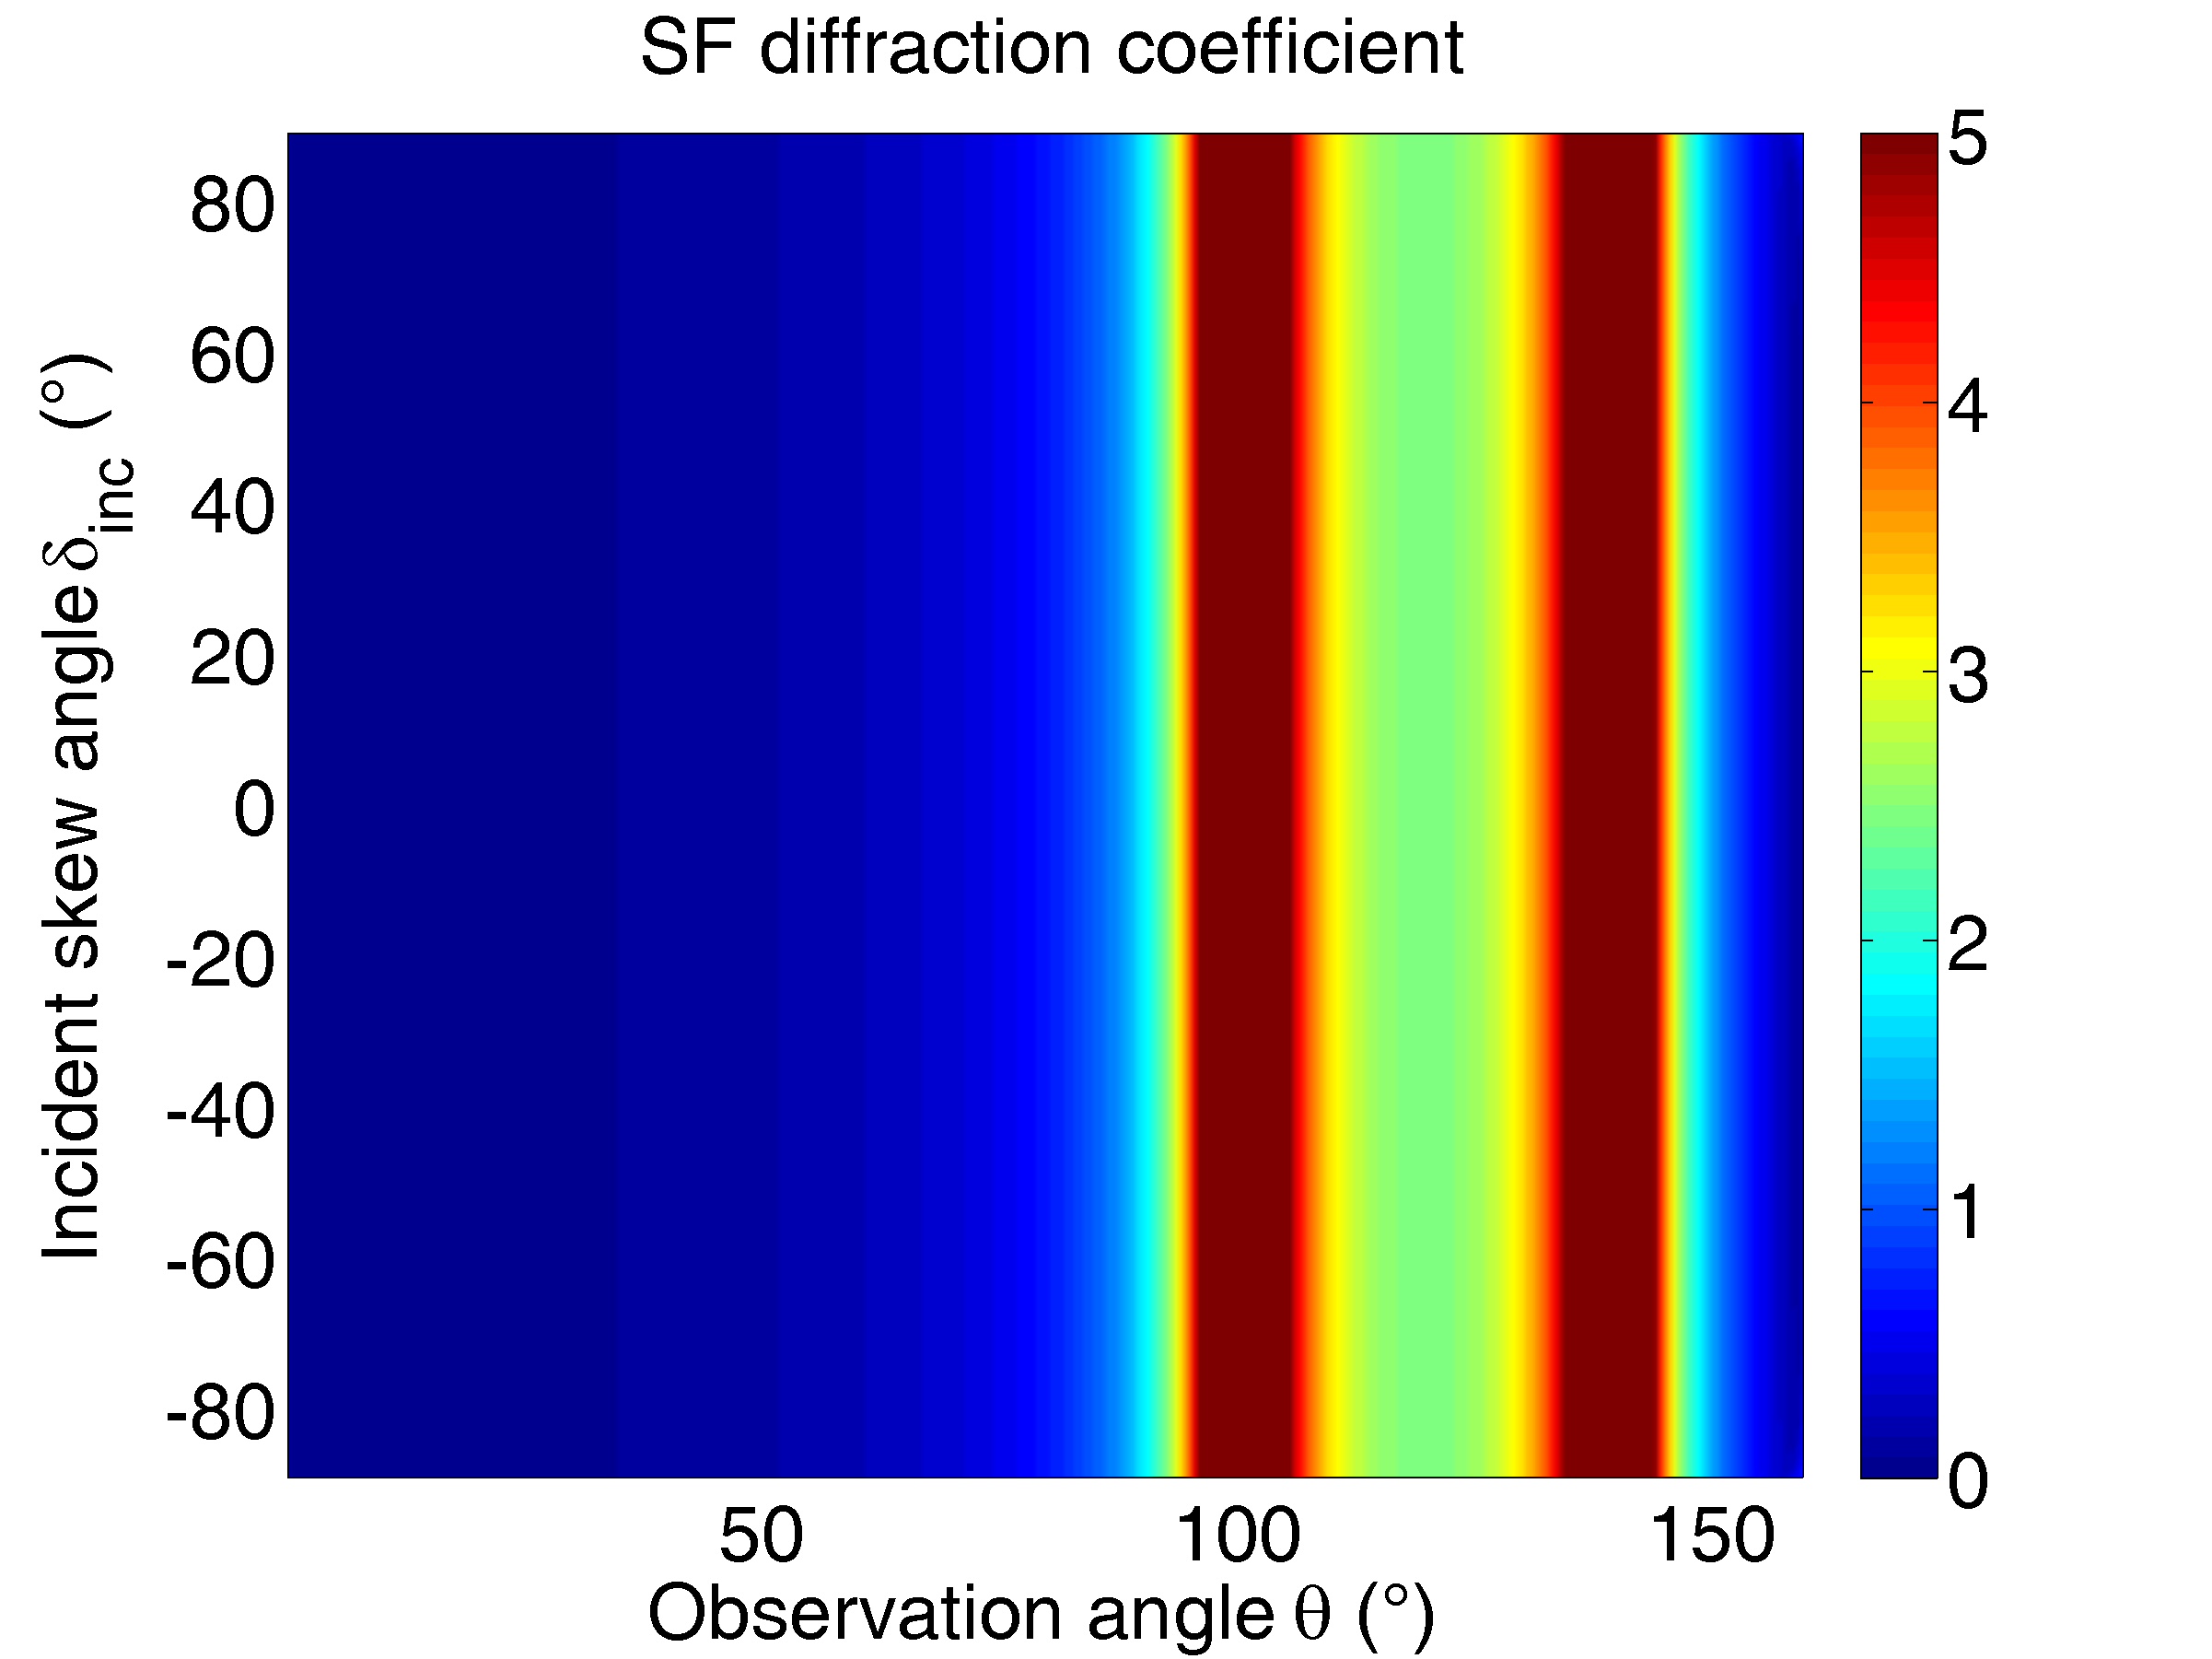
\includegraphics[width=\textwidth]{images/chapter4/Xprop_160_40.png}
        \caption{\acrshort{sf} diffraction coefficient}
        \label{C4:acSF16040}
    \end{subfigure}
\begin{subfigure}[b]{0.49\textwidth}
        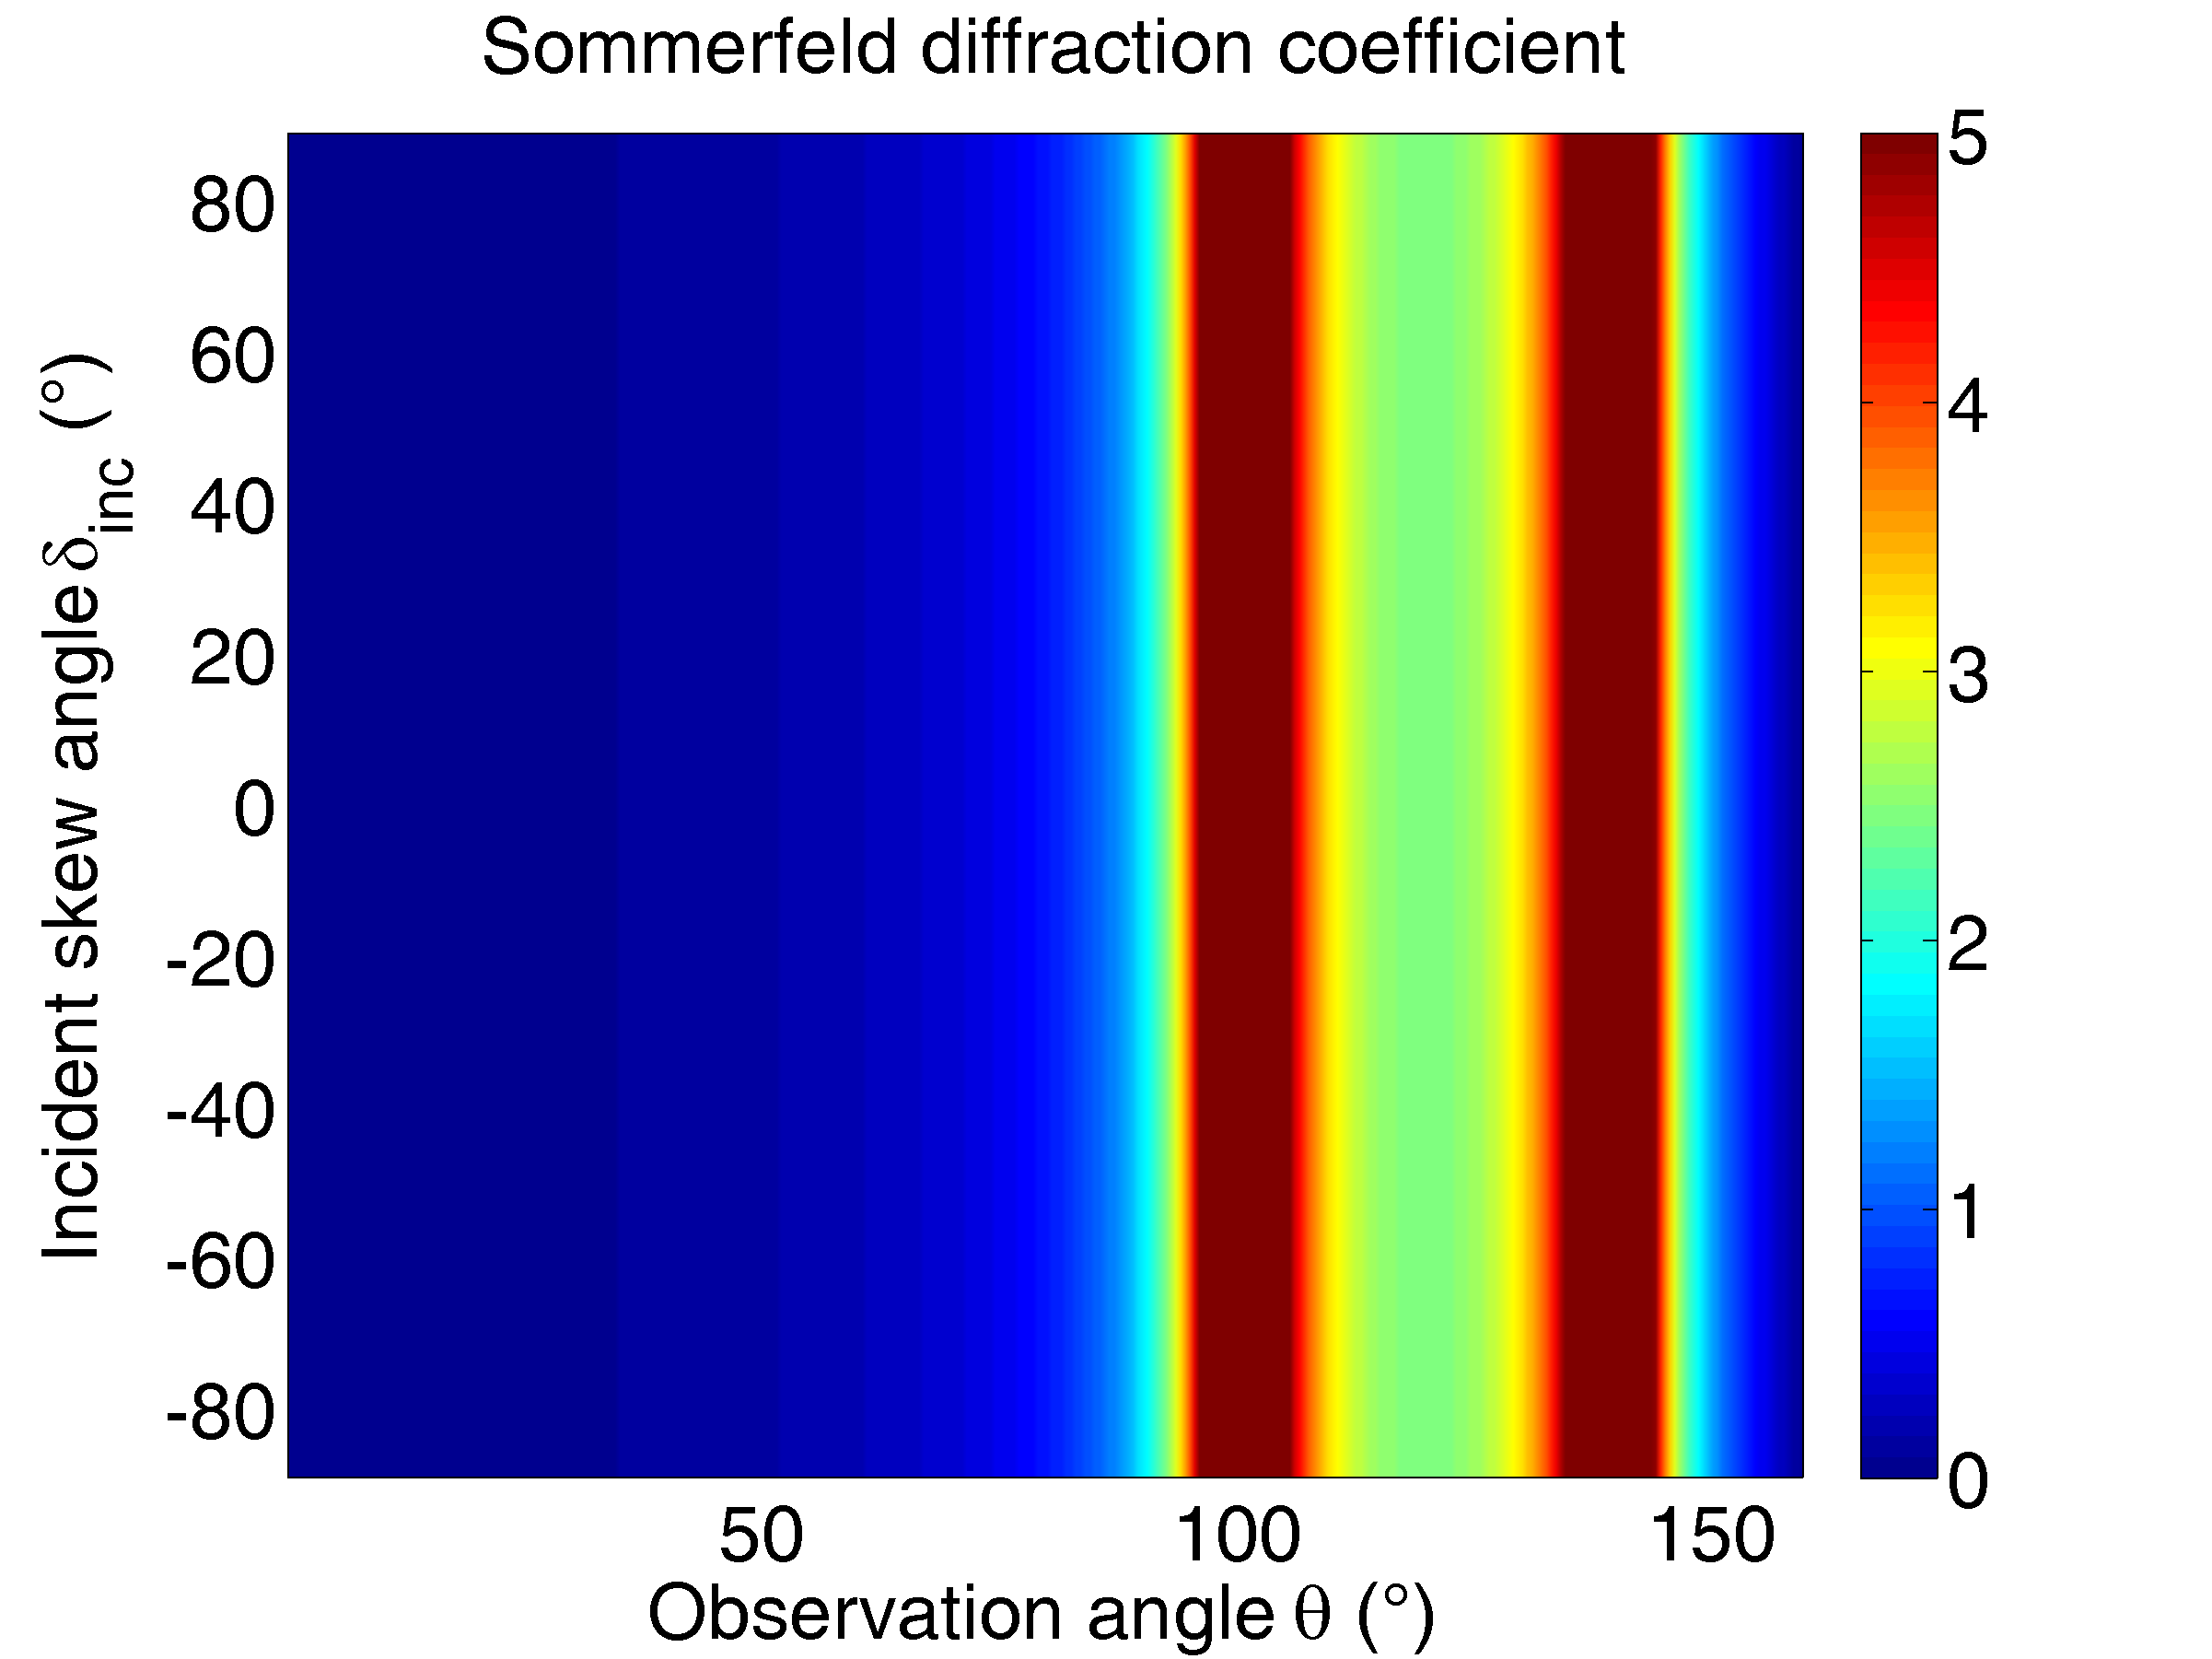
\includegraphics[width=\textwidth]{images/chapter4/Sommerfeld_160_40.png}
        \caption{Sommerfeld diffraction coefficient}
        \label{C4:Som16040}
    \end{subfigure}
\caption{Absolute value of the diffraction coefficient computed with the spectral functions and with the Sommerfeld method for a wave incident with and angle $\theta_{inc}=40^o$ on a wedge of angle $\varphi=160^o$}
\label{C4:ac16040}
\end{figure}

\begin{figure}
\centering
\begin{subfigure}[b]{0.49\textwidth}
        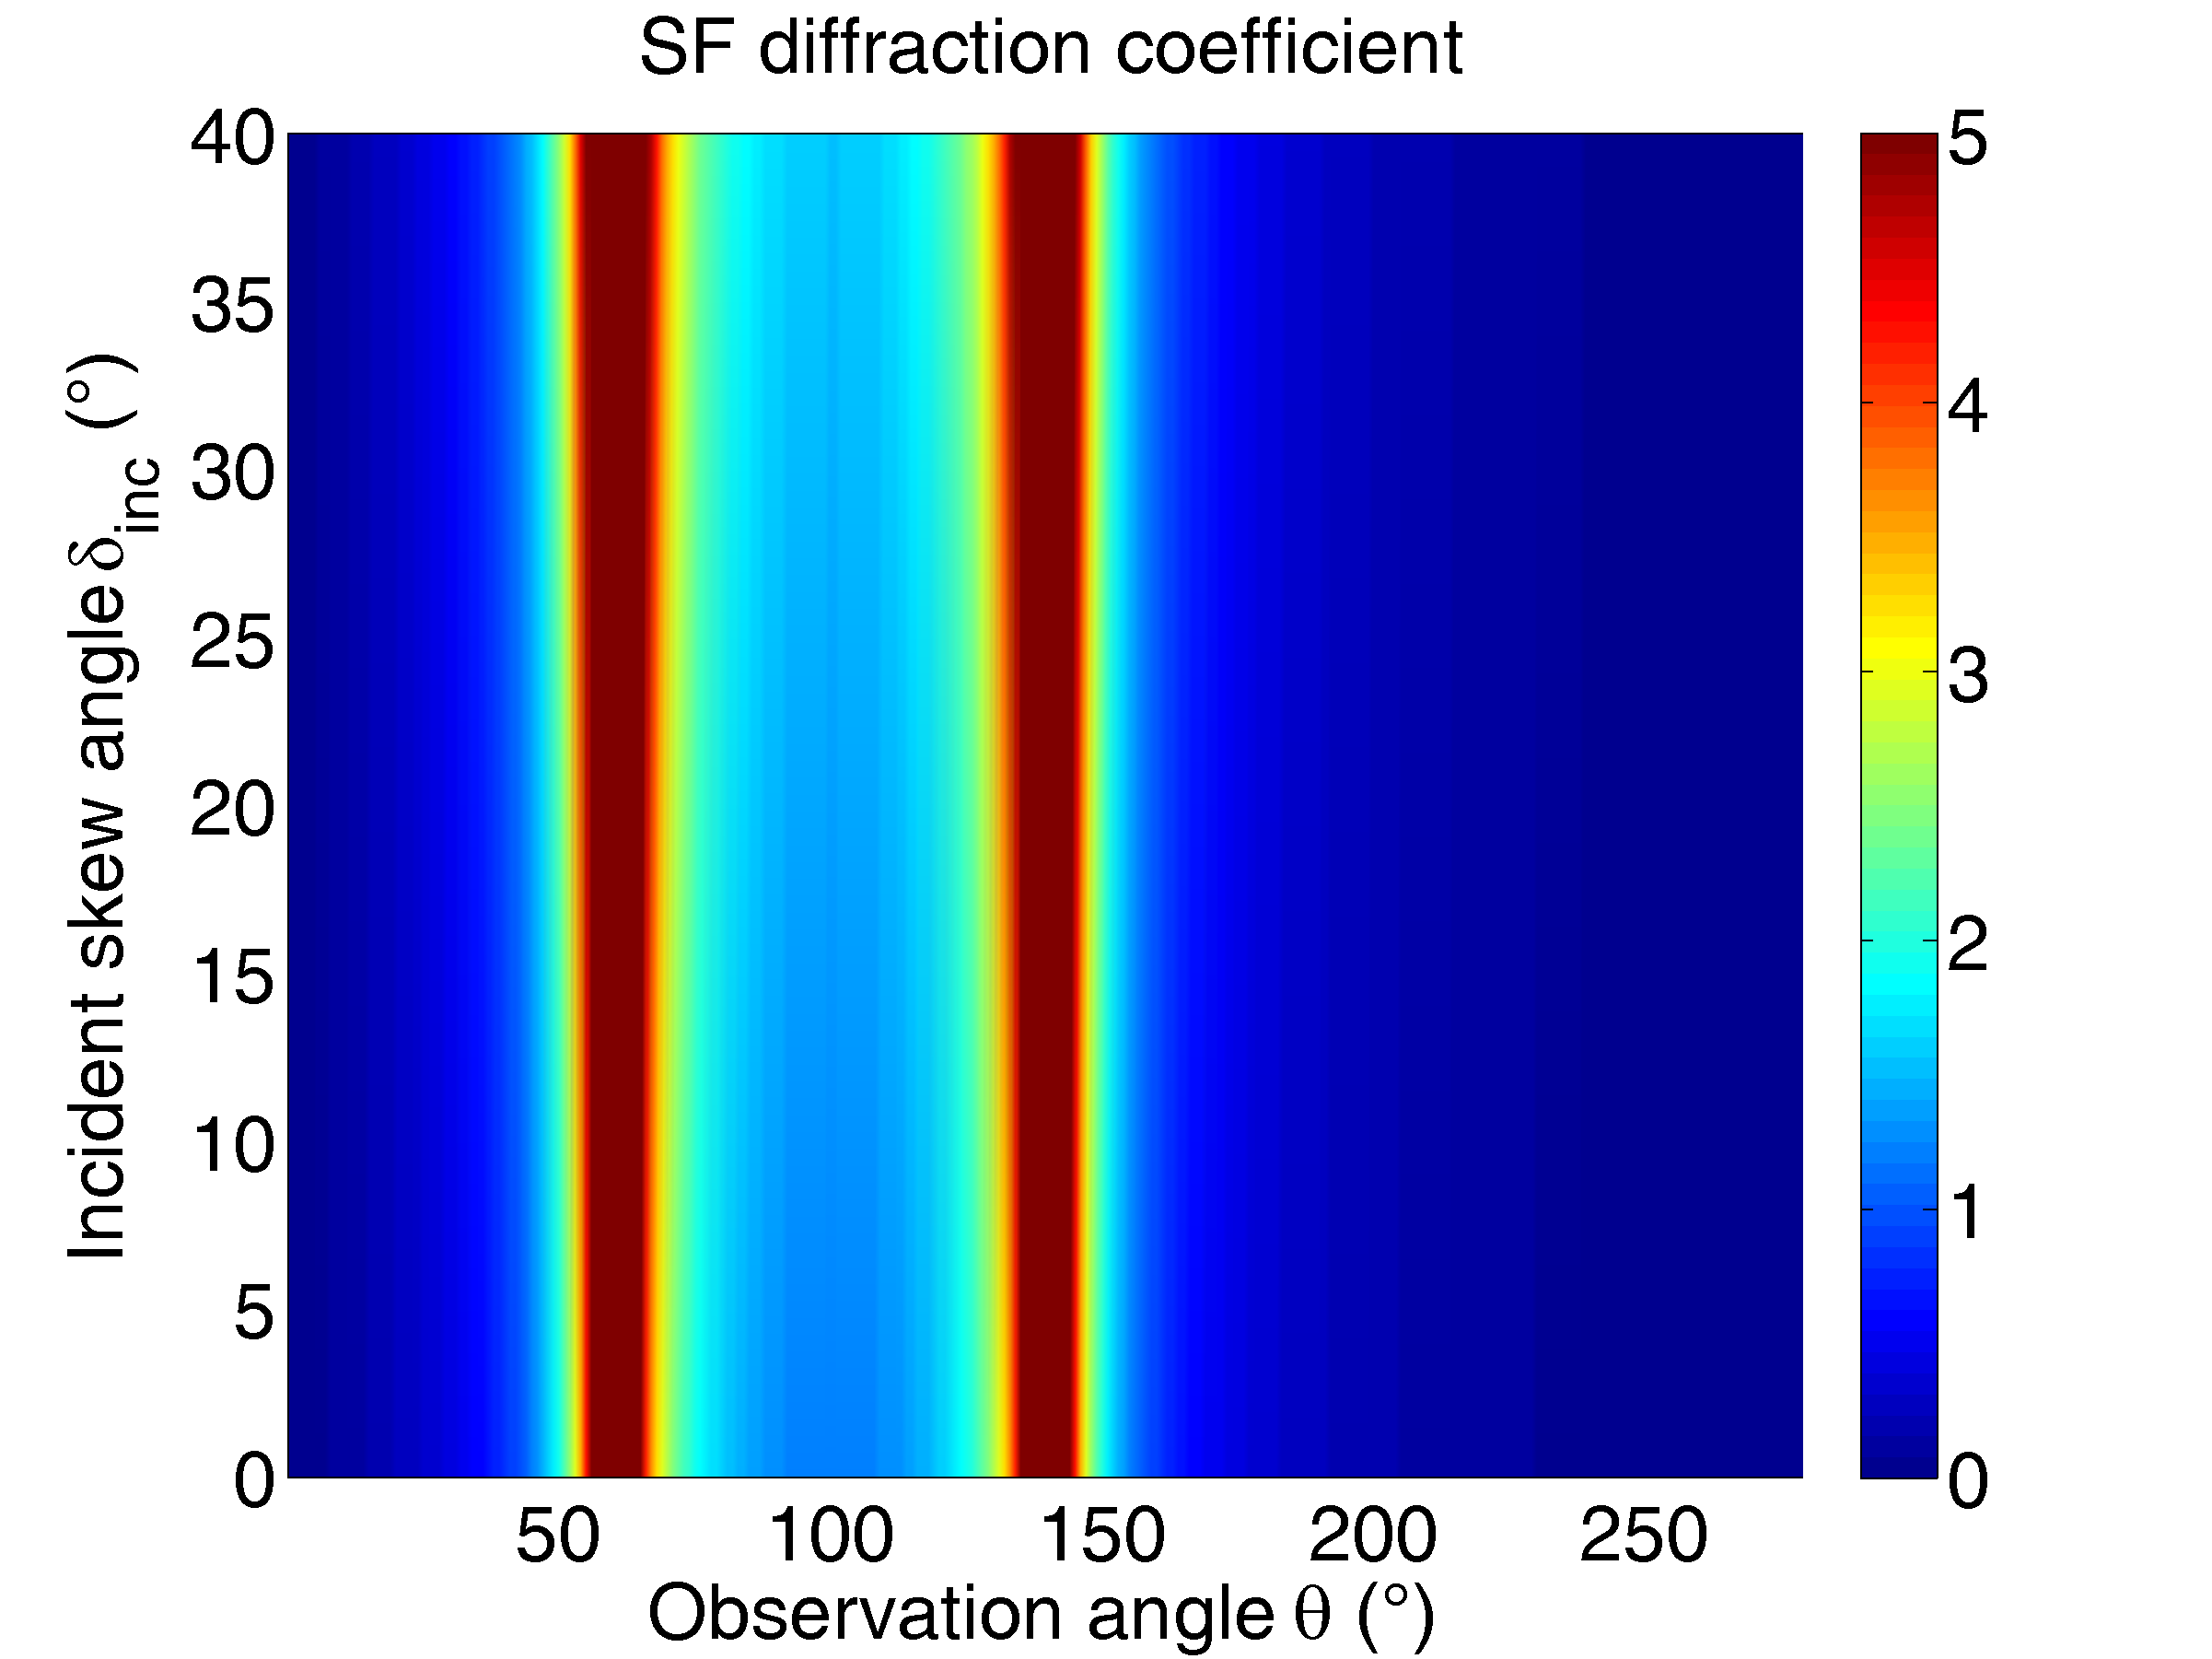
\includegraphics[width=\textwidth]{images/chapter4/Xprop_280_239.png}
        \caption{\acrshort{sf} diffraction coefficient}
        \label{C4:ac280240}
    \end{subfigure}
\begin{subfigure}[b]{0.49\textwidth}
        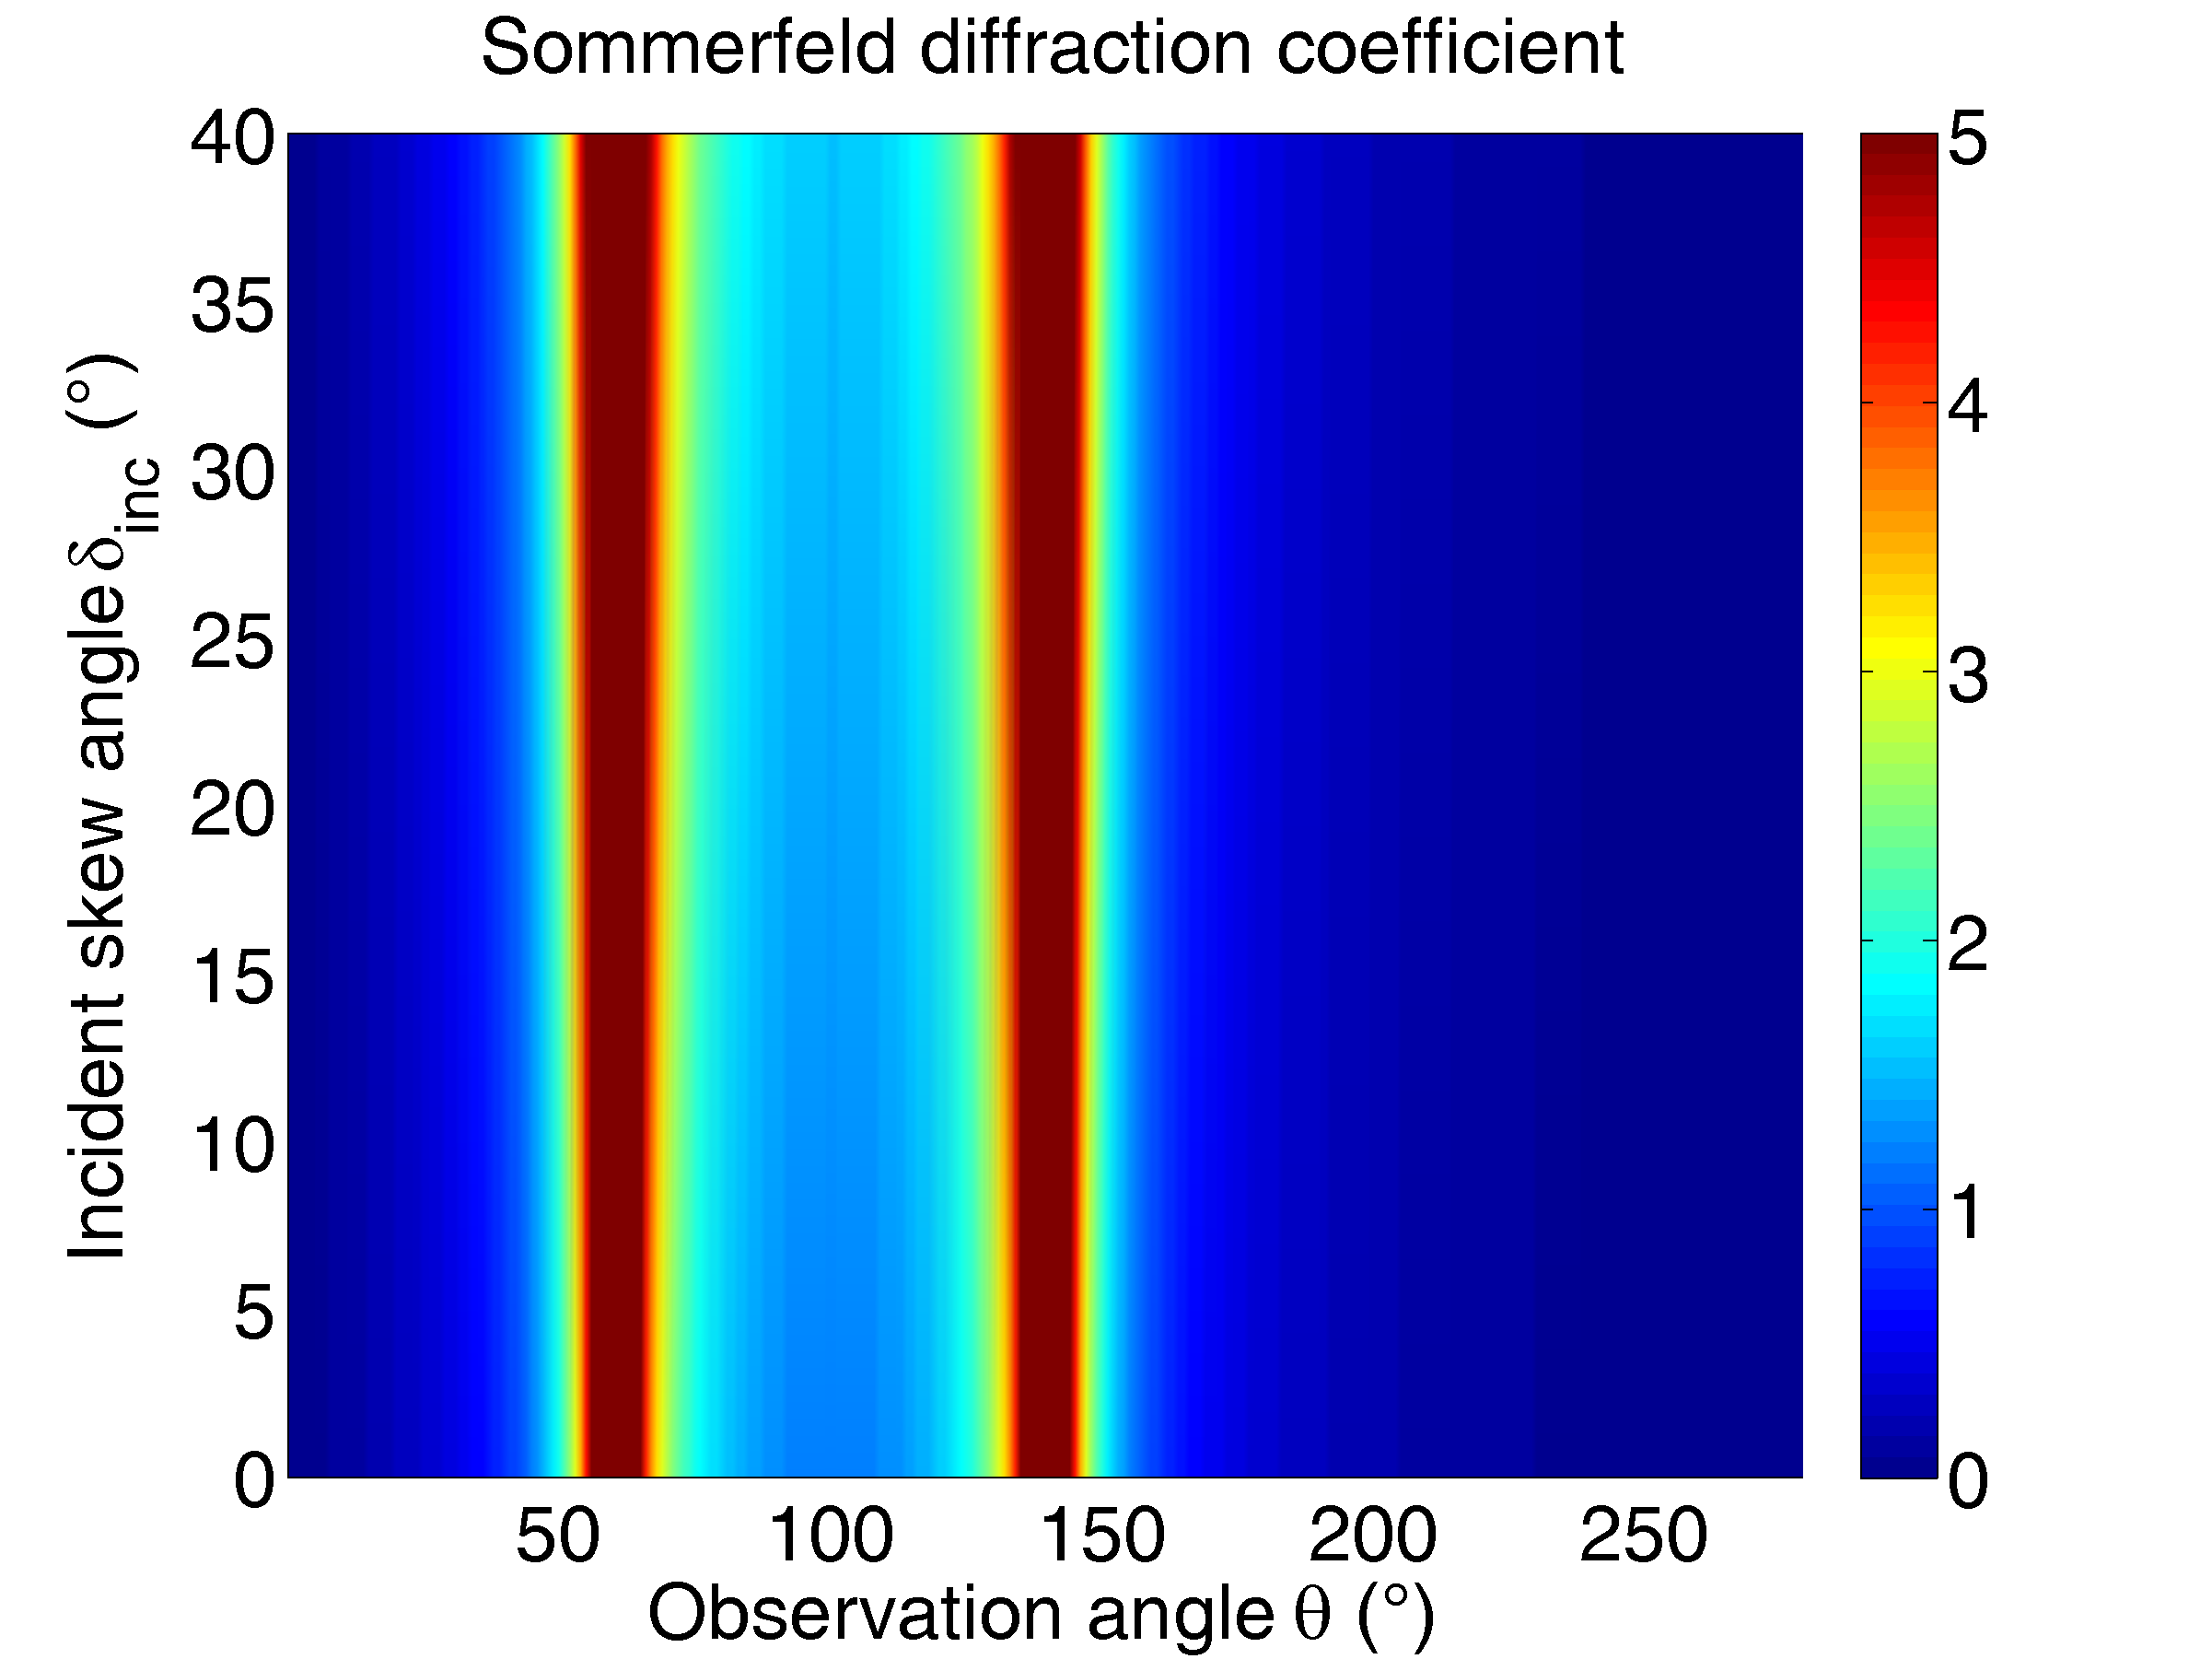
\includegraphics[width=\textwidth]{images/chapter4/Sommerfeld_280_239.png}
        \caption{Sommerfeld diffraction coefficient}
        \label{C4:Som280240}
    \end{subfigure}
\caption{Absolute value of the diffraction coefficient computed with the spectral functions and with the Sommerfeld method for a wave incident with and angle $\theta_{inc}=240^o$ on a wedge of angle $\varphi=280^o$}
\label{C4:ac280240}
\end{figure}

\begin{figure}
\centering
\begin{subfigure}[b]{0.49\textwidth}
        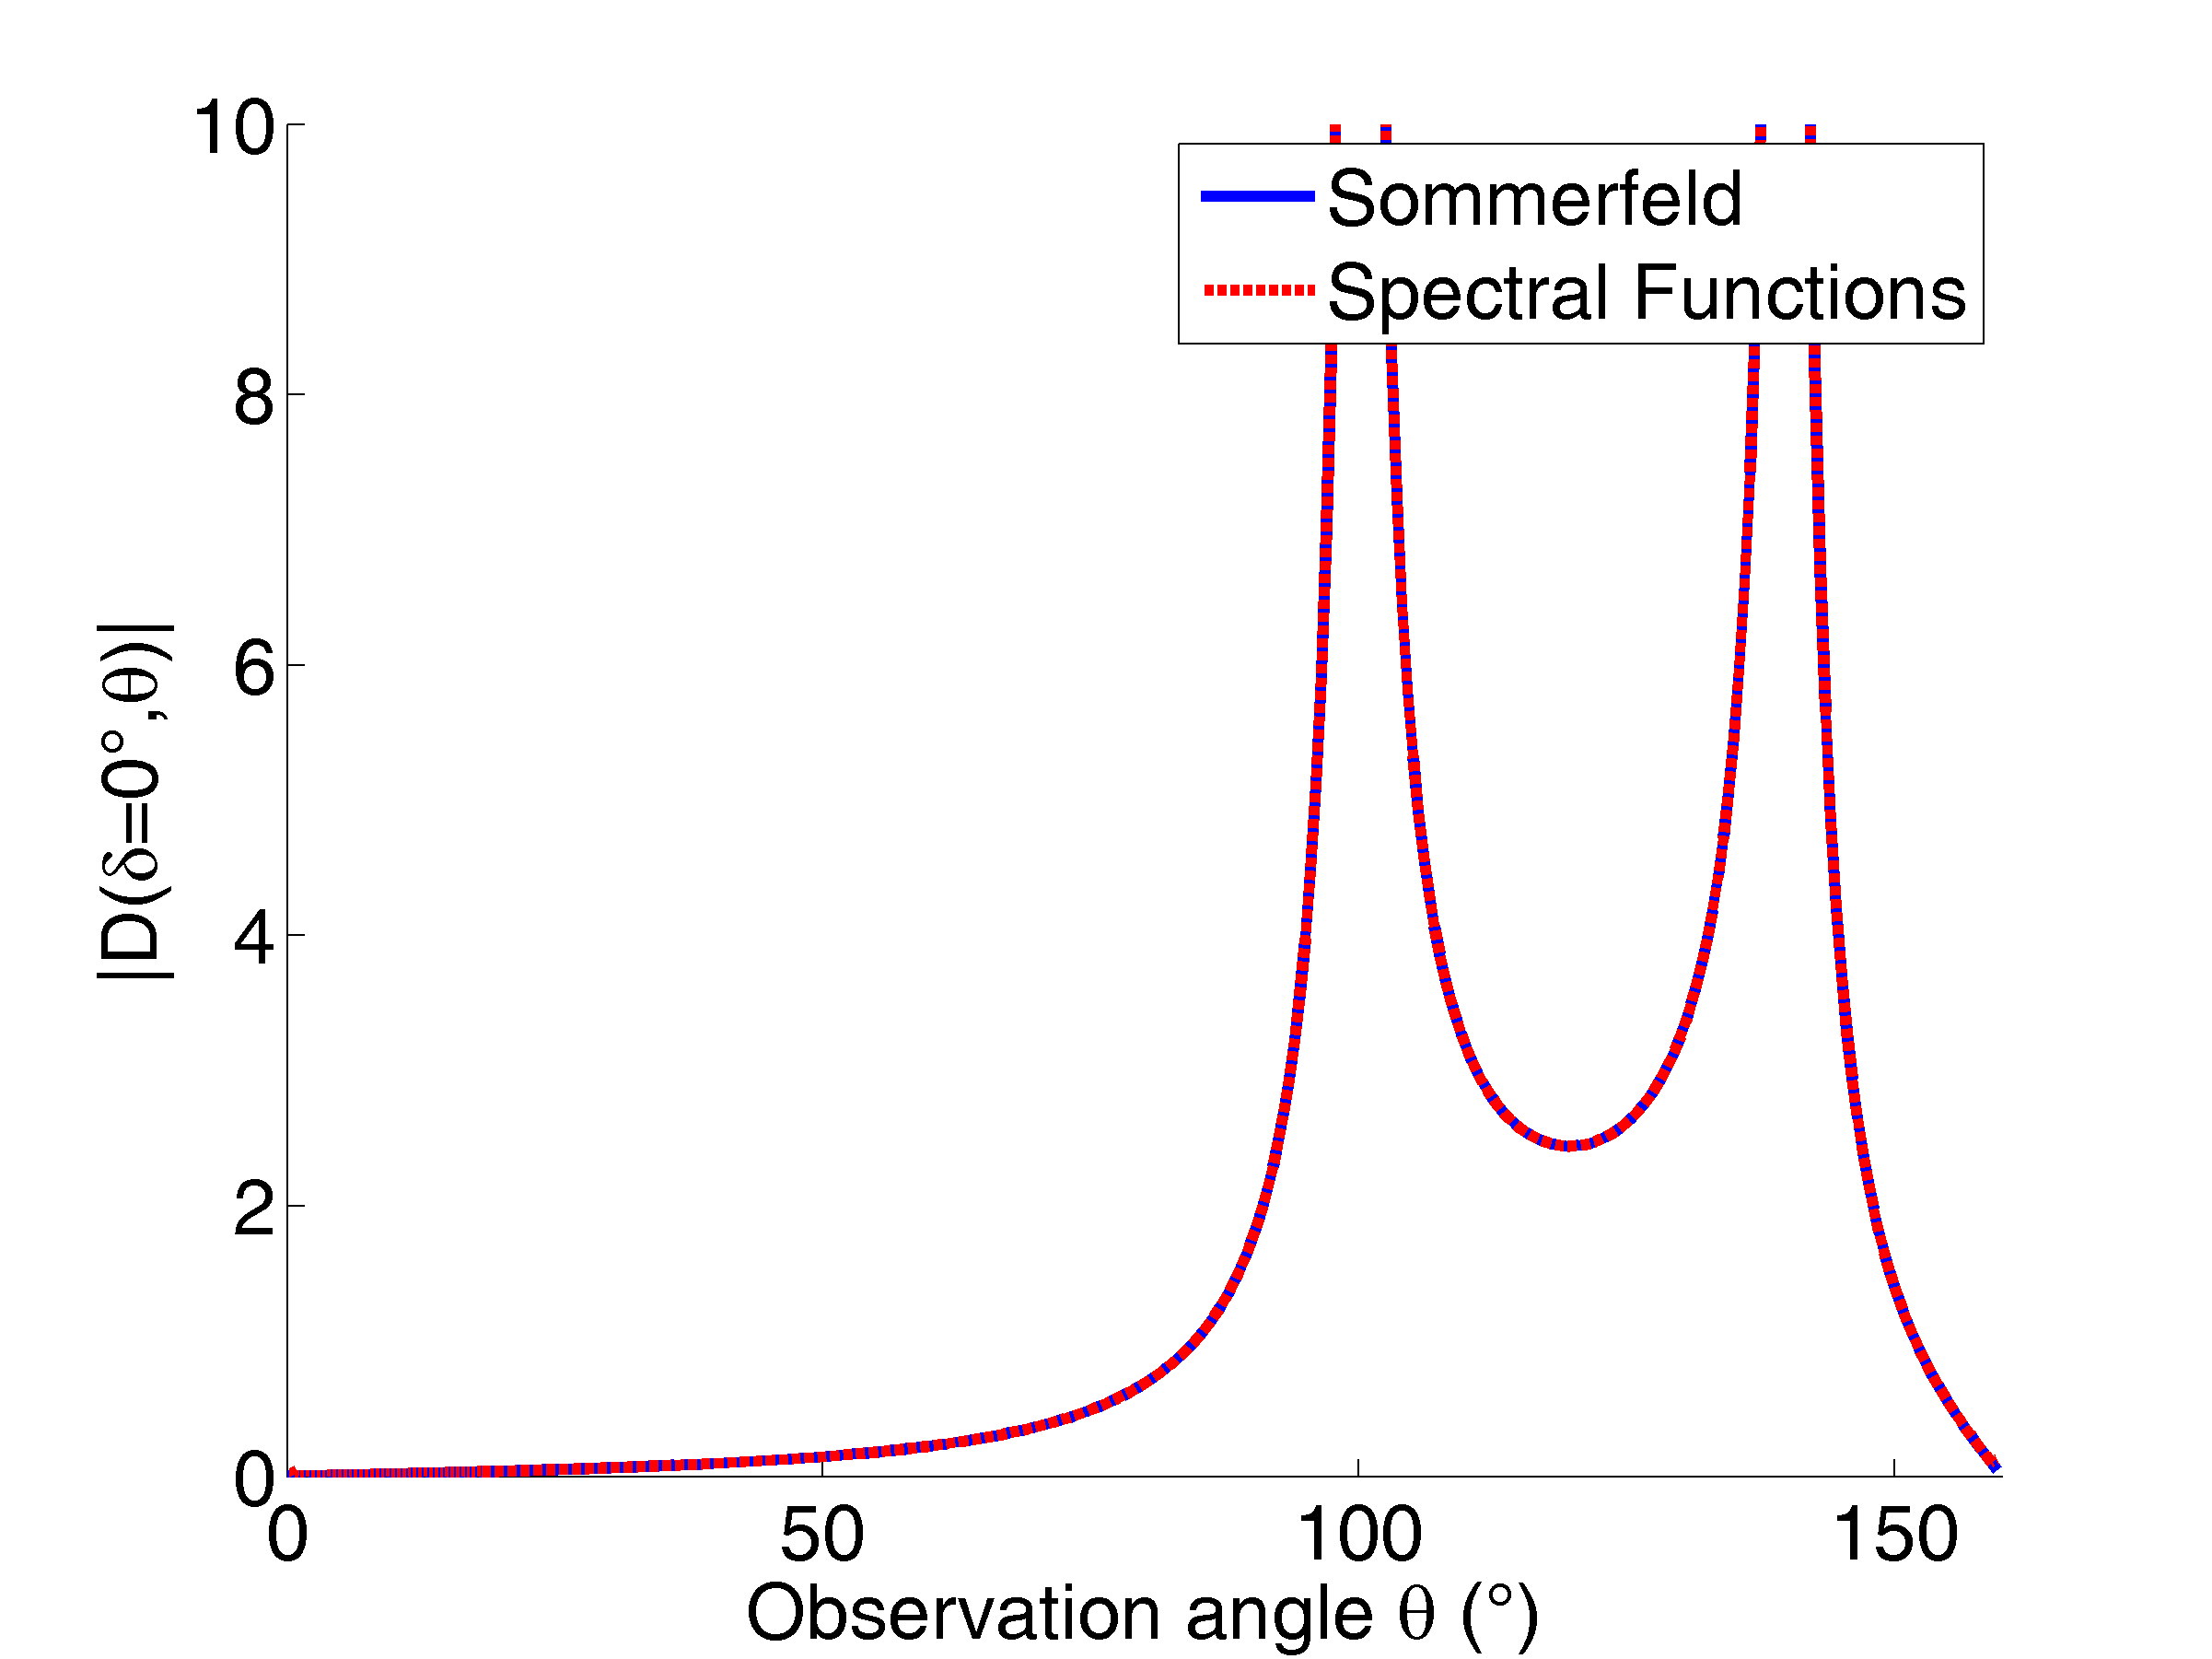
\includegraphics[width=\textwidth]{images/chapter4/D_160_40_0.png}
        \caption{$\theta_{inc}=40^o, \, \, \varphi=160^o$}
        \label{C4:ac280240}
    \end{subfigure}
\begin{subfigure}[b]{0.49\textwidth}
        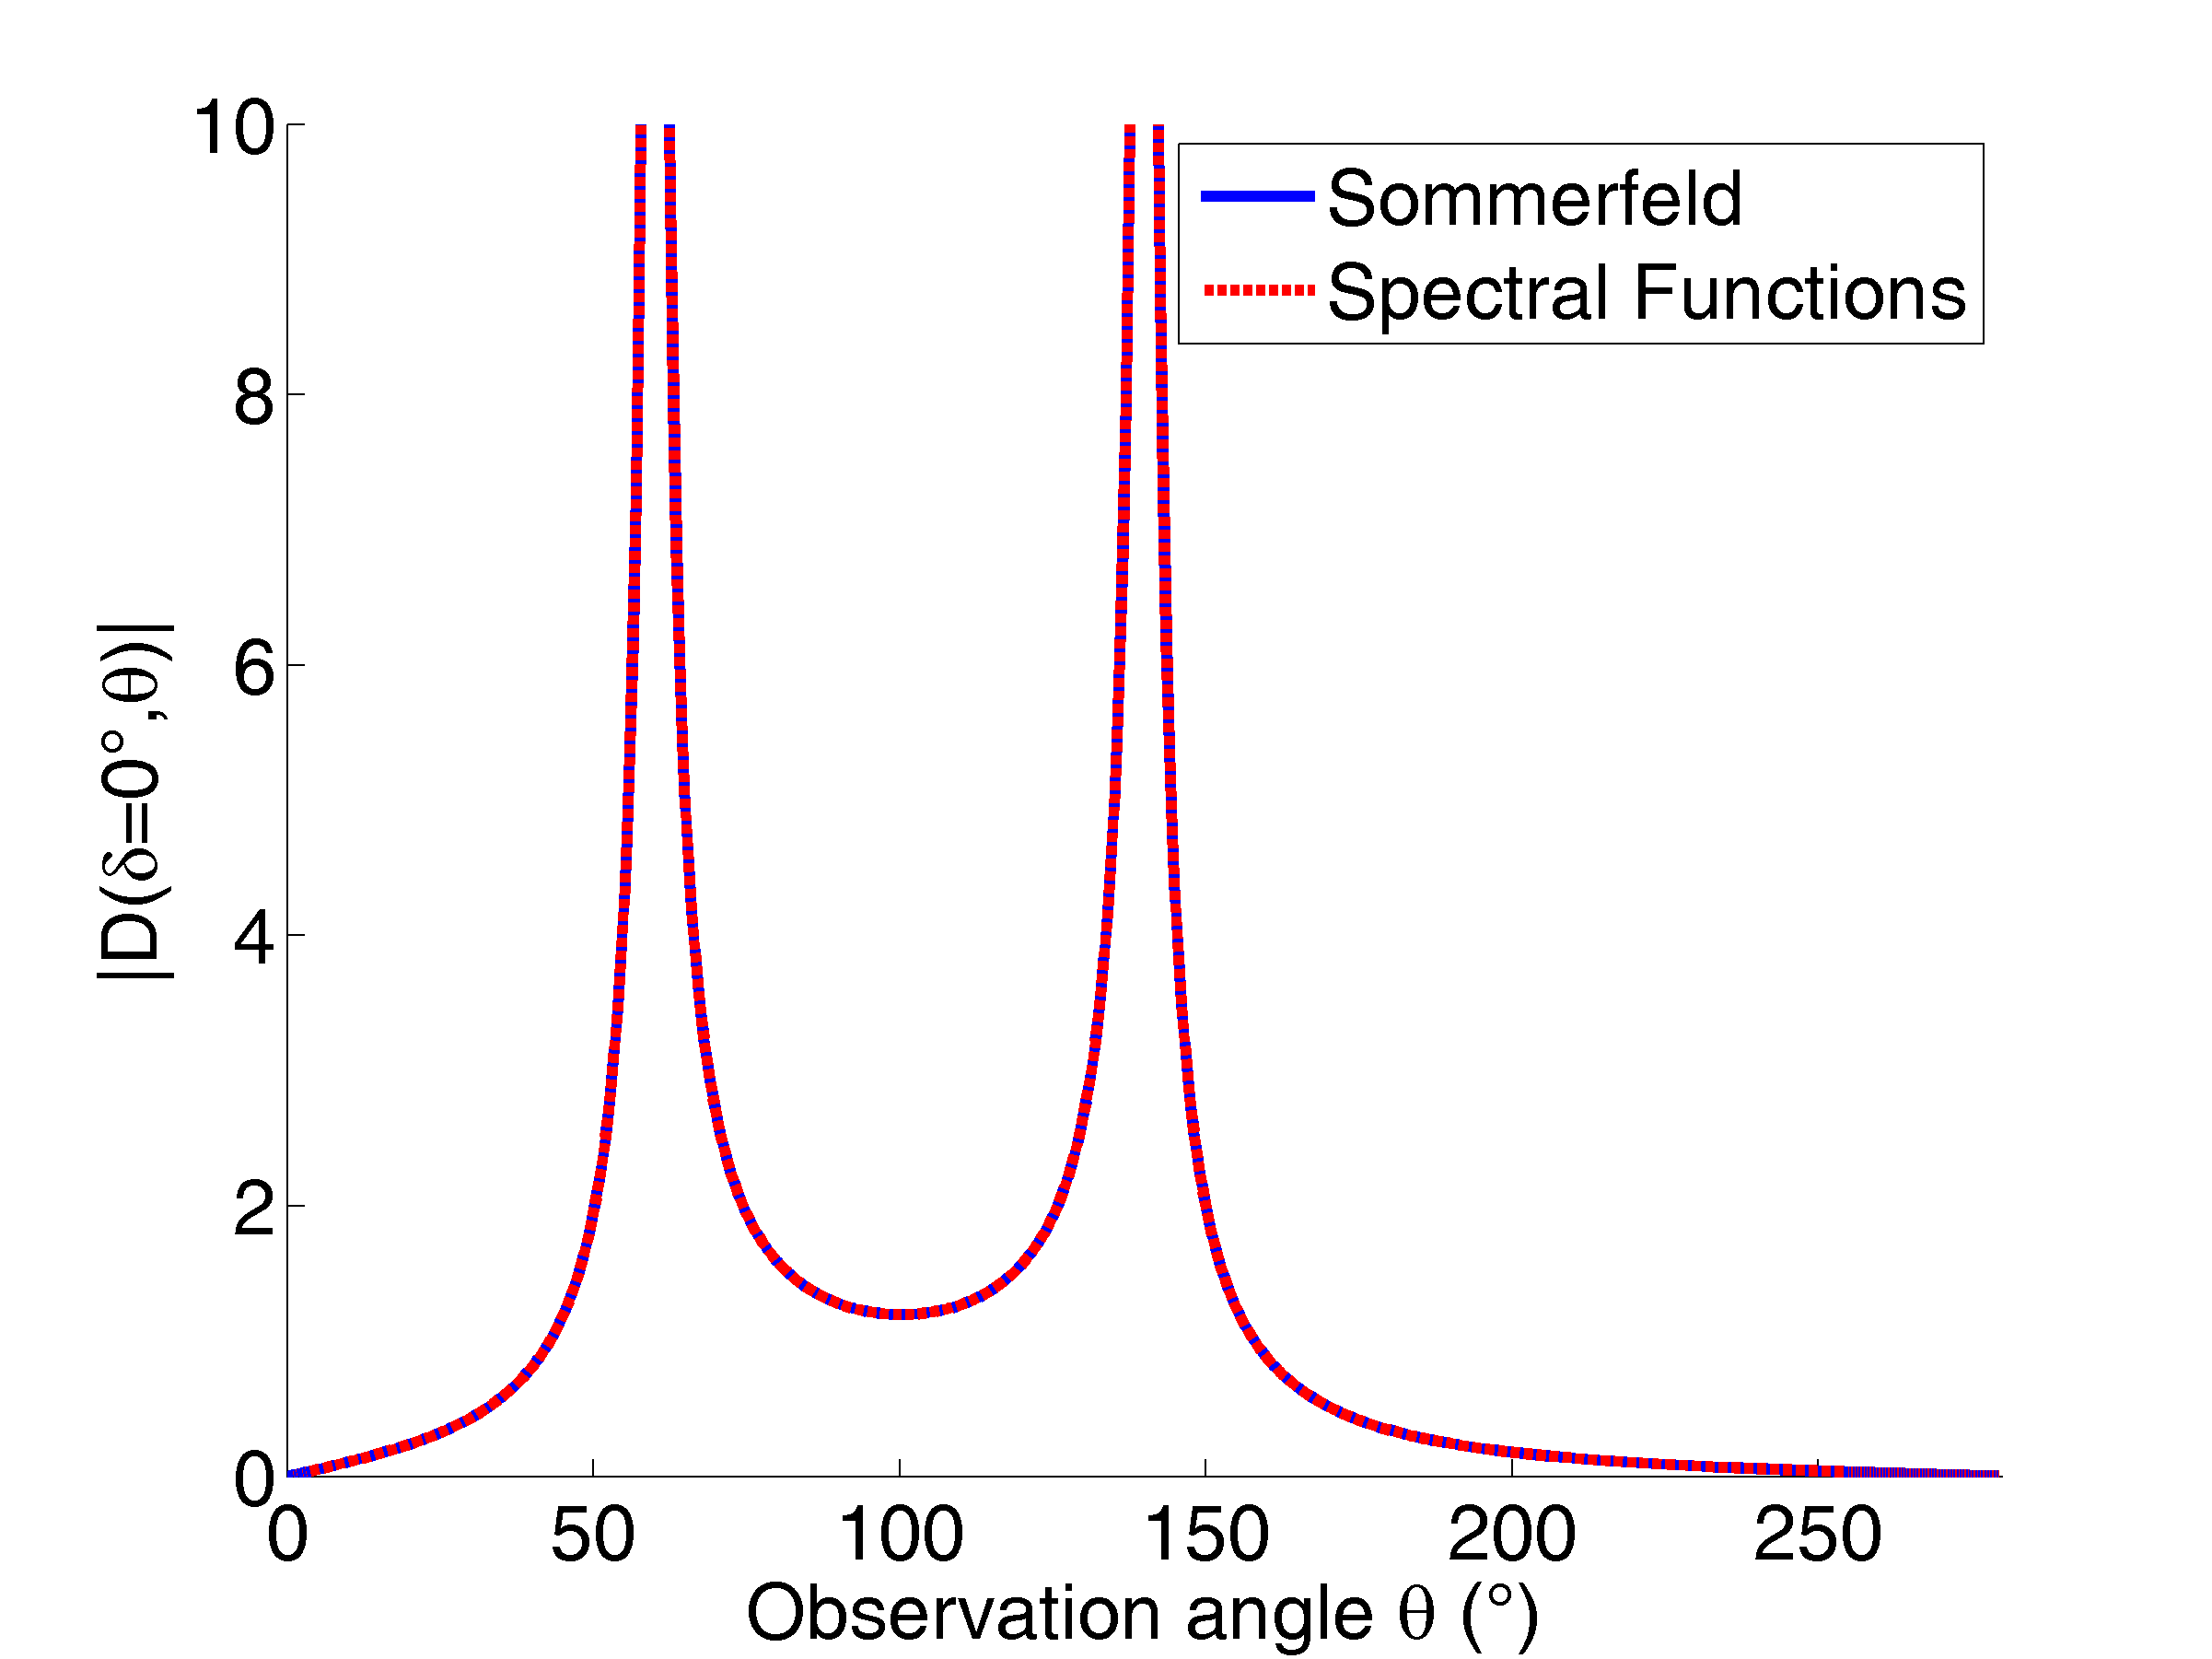
\includegraphics[width=\textwidth]{images/chapter4/D_280_239_0.png}
        \caption{$\theta_{inc}=240^o, \, \, \varphi=280^o$}
        \label{C4:Som280240}
    \end{subfigure}
\caption{Absolute value of the diffraction coefficient computed with the spectral functions and with the Sommerfeld method for $\delta_{inc}=0^o$.}
\label{C4:ac280240}
\end{figure}

Comparing our results to Sommerfeld's analytical formulation, provides an additional check on the results.

\subsection{Case where $\crit$}
In the case where $\crit$, the code developed according to the theory described in this chapter produces diverging results. Additional work is necessary in order to solve this problem. In the meantime, in order to obtain coherent results, the following approximation is applied :
\begin{equation}
X_j|_{\delta_{\beta}>\delta_C} \approx X_j|_{\delta_{\beta}=\delta_C-\epsilon}
\end{equation}

\section*{Conclusion}
Using the spectral functions method, the elastic wave diffracted by a skew incident plane wave on as stress-free wedge has been studied. In cases where Snell's law of diffraction has a solution for both longitudinal and transversal diffracted waves, a semi-analytical computation method is developed theoretically and numerically. The corresponding code has been checked in three different manners, yielding promising results. In the case of an incident transversal wave, with a skew angle higher than the critical angle in diffraction, Snell's law of diffraction leads only to transversal diffracted waves. This case is also treated theoretically but the corresponding numerical code produces diverging results. Further investigations are necessary in order to solve this problem. In the meantime, an approximate solution is proposed, in order to obtain a less exact, yet physically meaningful result. This approximate solution still remains to be tested.
